\chapter{The Response to Phenotypic Selection}
\marginnote{See \citet{lewontin1970units}. Note that these
  requirements are not specific to DNA, i.e. the concept of
  evolution by natural selection is substrate independent. }
Evolution by natural selection requires:
\begin{enumerate}
\item Variation in a phenotype
\item That survival is non-random with respect to this phenotypic
variation.
\item That this variation is heritable.
\end{enumerate}
Points 1 and 2 encapsulate our idea of Natural Selection, but evolution by natural
selection will only occur if the 3rd condition is also
met. \sidenote{Some people consider natural selection to only operate on heritable phenotype varation
  and so require all three conditions to say that natural selection
  occurs. This is mostly a semantic point, however, it is useful to be
able to distinguish the action of selection from a possible response.} It is the
heritable nature of variation that couples change within a generation
due to natural selection to change across generations (evolutionary
change). \\

Let's start by thinking about the change within a generation due
to directional selection, where selection acts to change the mean
phenotype within a generation. For example, a decrease in mean height within a
generation, due to taller organisms having a lower chance of surviving
to reproduction than shorter organisms. Specifically, we'll denote our mean phenotype at
reproduction by $\mu_S$, i.e. after selection has acted, and our mean
phenotype before selection acts by $\mu_{BS}$. This second quantity may be hard to
measure, as obviously selection acts throughout the life-cycle, so it
might be easier to think of this as the mean phenotype if selection
hadn't acted. So the change in mean phenotype within a generation is $\mu_{S} - \mu_{BS}= S$.  \\

\begin{marginfigure}
\begin{center}
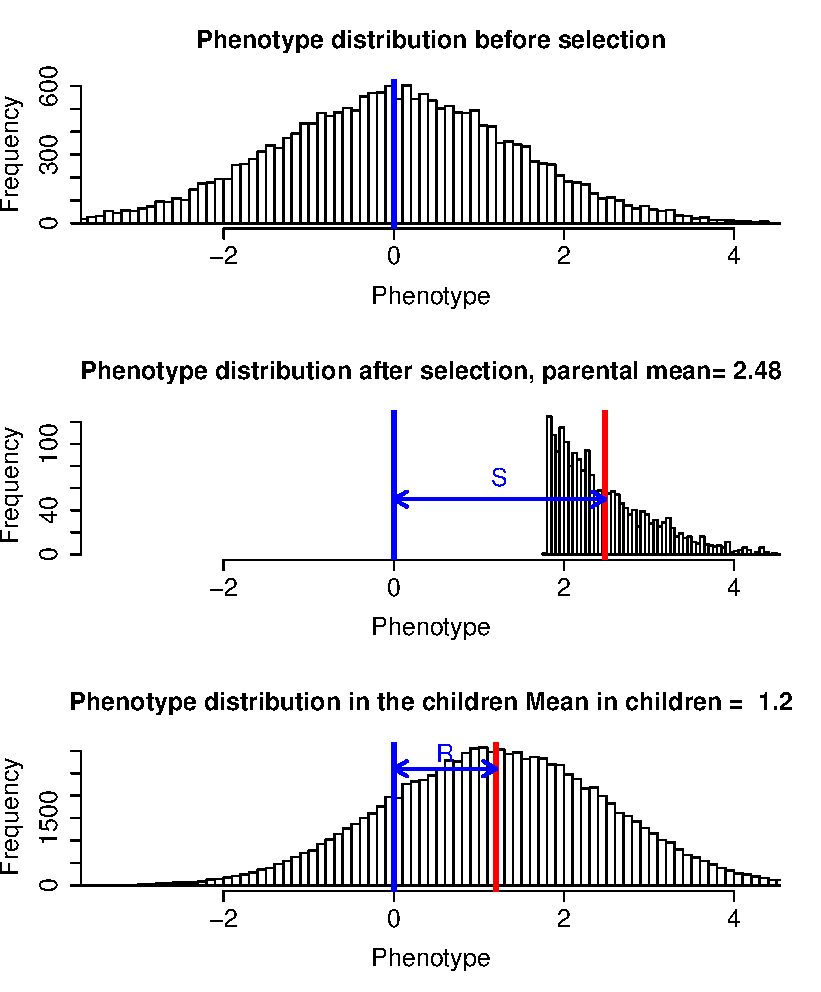
\includegraphics[width=\textwidth]{figures/Response_to_sel/QT3.pdf}
\end{center}
\caption{{\bf Top.} Distribution of a phenotype in the parental population
  prior to selection, $V_A=V_E=1$. {\bf Middle.} Only individuals in the top $10\%$
  of the phenotypic distribution are selected to reproduce; the resulting shift
  in the phenotypic mean is $S$. {\bf Bottom.}  Phenotypic distribution of
  children of the selected parents; the shift in the mean phenotype is
$R$. \gitcode{https://github.com/cooplab/popgen-notes/blob/master/Rcode/Quant_gen/QT3.R}}
\end{marginfigure}

We are interested in predicting the distribution of phenotypes in the next
generation. In particular, we are interested in the mean phenotype in
the next generation to understand how directional selection has
contributed to evolutionary change. We'll denote the mean phenotype in
offspring, i.e. the mean phenotype in the next generation before selection acts,
as $\mu_{NG}$. The change across generations we'll call the response
to selection $R$ and put this equal to $\mu_{NG}- \mu_{BS}$. \\


The mean phenotype in the next generation is
\begin{equation}
\mu_{NG} = \E \left( \E(X_{kid} | X_{mum},X_{dad}) \right)
\end{equation}
where the outer expectation is over possible pairs of randomly mating individuals
who survive to reproduce. We can use eqn. \ref{predict_kid} to obtain
an expression for this expectation:
\begin{equation}
\mu_{NG} = \mu_{BS} +
\beta_{mid,kid} ( \E(X_{mid}) - \mu_{BS})
\end{equation}

\begin{marginfigure}
\begin{center}
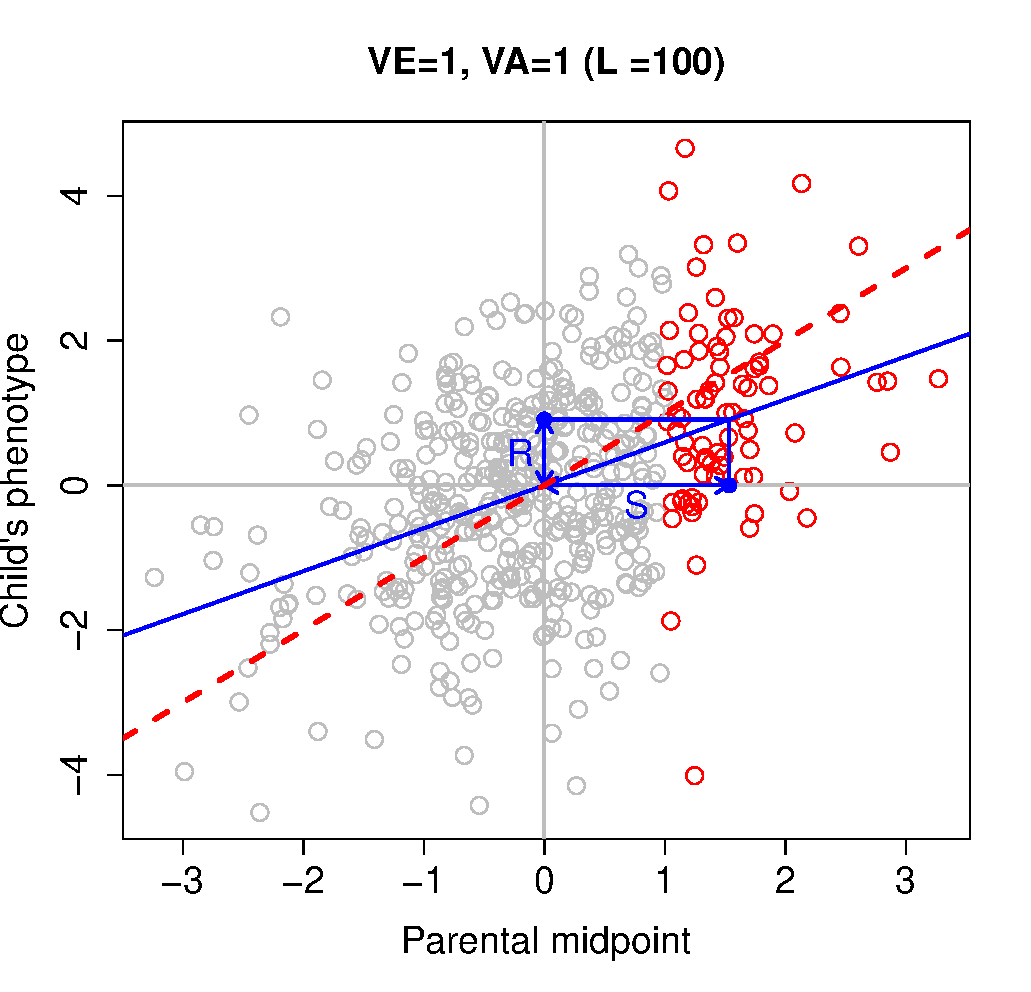
\includegraphics[width=\textwidth]{figures/Response_to_sel/Breeders_eqn.pdf}
\end{center}
\caption{A visual representation of the Breeder's equation. Regression of child's phenotype on parental mid-point phenotype ($V_A=V_E=1$). Under truncation selection, only individuals
  with phenotypes $>1$ (red) are bred. \gitcode{https://github.com/cooplab/popgen-notes/blob/master/Rcode/Quant_gen/QT2.R}}
\end{marginfigure}

So to obtain $\mu_{NG}$ we need to compute $\E(X_{mid})$, the expected
mid-point phenotype of pairs of individuals who survive to
reproduce. Well this is just the expected phenotype in the individuals
who survived to reproduce ($\mu_{S}$), so
\begin{equation}
\mu_{NG} = \mu_{BS} +
h^2 (\mu_S - \mu_{BS})
\end{equation}
So we can write our response to selection as
\begin{equation}
R = \mu_{NG} -\mu_{BS}  =
h^2 (\mu_S - \mu_{BS}) = h^2 S \label{breeders_eqn}
\end{equation}
So our response to selection is proportional to our selection
differential, and the constant of proportionality is the narrow sense
heritability. This equation is sometimes termed the Breeder's
equation. It is a statement that the evolutionary change across
generations ($R$) is proportional to the change caused by directional selection
within a generation ($S$), and that the strength of this relationship is
determined by the narrow sense heritability ($h^2$). \\

%\graham{Lost the barncle question, put it back in.}



\begin{figure}
\begin{center}
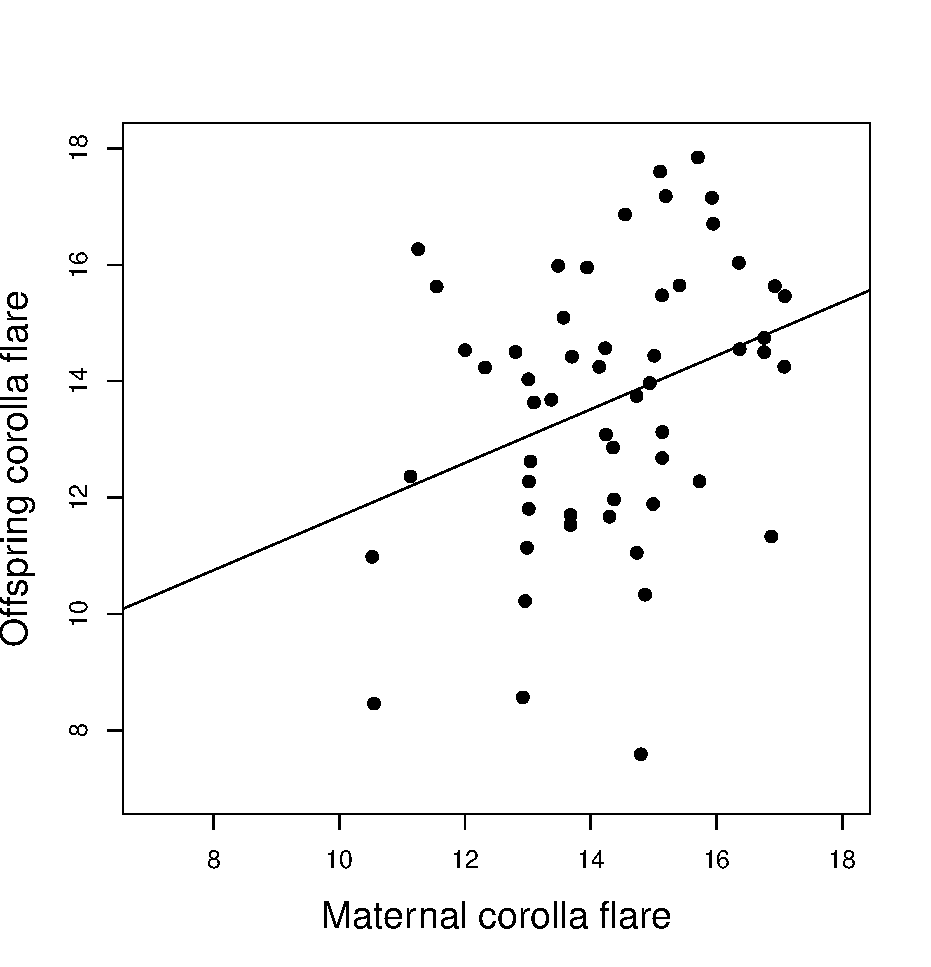
\includegraphics[width= 0.6 \textwidth]{Journal_figs/Quant_gen/Galen_flower_herit/Galen_corolla_flare.pdf} 
\end{center}
\caption{The relationship between maternal and offspring corolla flare (flower
  width) in P. viscosum. From \citeauthor{galen:96}'s data the
  covariance of mother and child is 1.3, while the variance of the
  mother is 2.8. Data from \citet{galen:96}. \gitcode{https://github.com/cooplab/popgen-notes/blob/master/Journal_figs/Quant_gen/Galen_flower_herit/Gallen_analysis.R}} \label{fig:Galen_corolla}  
\end{figure}

\begin{marginfigure}
\begin{center}
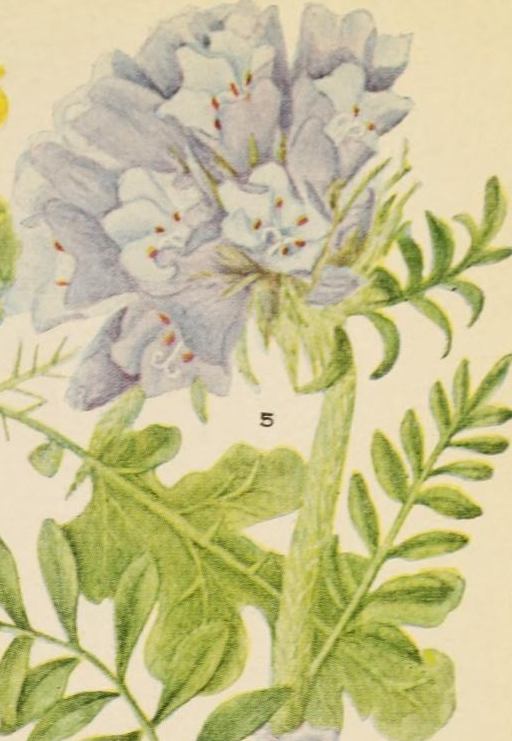
\includegraphics[width=0.75\textwidth]{illustration_images/Quant_gen/Polemonium_viscosum_Galen/Polemonium_viscosum.jpg}
\end{center}
\caption{Sticky jacob's ladder ({\it Polemonium viscosum}). \BHLNC{Flowers of Mountain and
    Plain (1920). Clements, E.}{https://www.biodiversitylibrary.org/page/40791993\#page/49/mode/1up}{New York Botanical Garden, Mertz Library}
Cropped from original.}
\end{marginfigure}


\begin{question}
\citet{galen:96} explored selection on flower shape in
{\it P. viscosum}.  She found that plants with larger corolla flare
had more bumblebee visits, which resulted in higher seed set and a
$17\%$ increase in corolla flare in the plants contributing to the
next generation. Based on the data in the caption of Figure \ref{fig:Galen_corolla}
what is the expected response in the next generation?
\end{question}

\begin{marginfigure}
\begin{center}
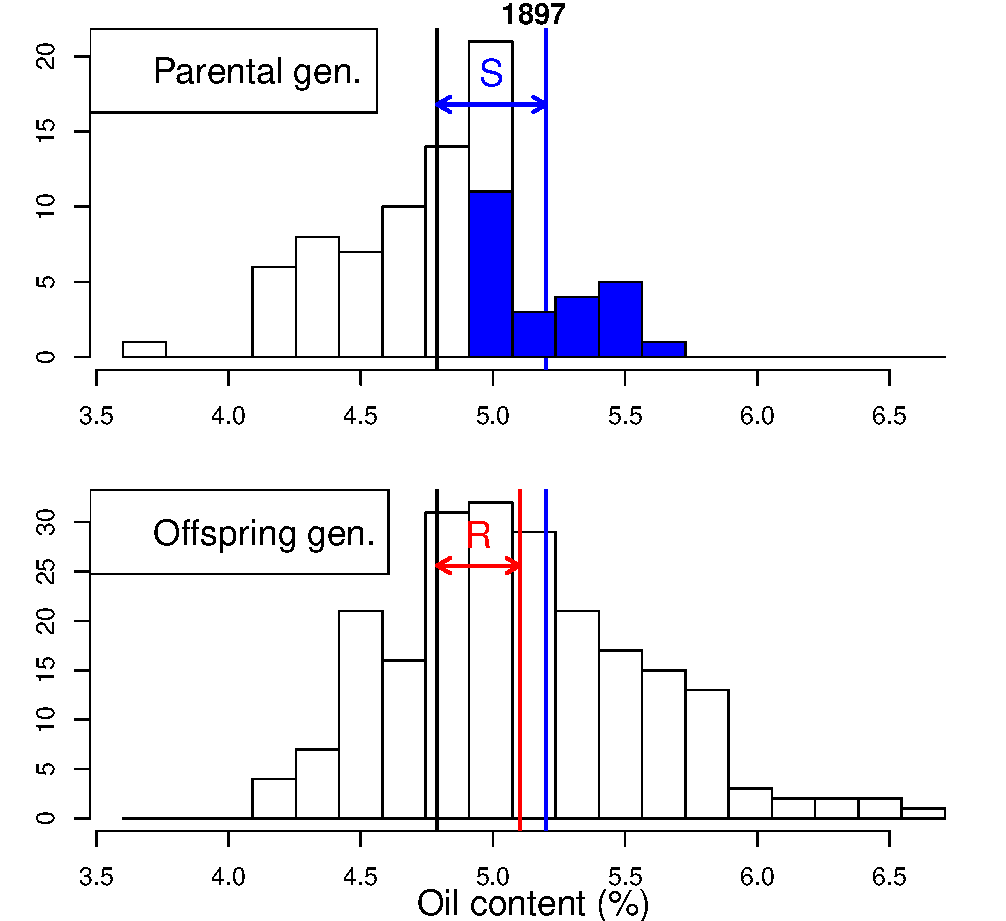
\includegraphics[width=\textwidth]{Journal_figs/Quant_gen/Illinois_long_term_selection_corn/Illinois_LTS_breeders_eq.pdf}
\end{center}
\caption{{\bf Top.} Phenotypic distribution of oil content in corn in
  1897, and the individuals who were selected to breed for the next
  generation are marked in blue.   {\bf Bottom.} The distribution in the next generation. Data from the
  Illinois selection experiment available \href{https://www.ideals.illinois.edu/handle/2142/3525}{here}, \gitcode{https://github.com/cooplab/popgen-notes/blob/master/Journal_figs/Quant_gen/Illinois_long_term_selection_corn/corn_LTS.R}}  \label{Fig:s}
\end{marginfigure}

If we know $R$ and $S$ we can estimate $h^2$. Heritabilities estimated
like this are called `realized heritability'. Estimates of the
`realized heritability' can readily be produced in artificial selection experiments, see for example Figure \ref{Illinois_LTS_breeders_eq}.
\begin{question}
  From the experiment shown in Figure \ref{Illinois_LTS_breeders_eq},
  the mean corn oil content in 1897 was $4.78$, among the $24$ individuals
chosen to breed to for the next generation the mean was $5.2$. The
offspring of these individuals in 1888 had a mean kernel oil content of
$5.1$. What is the narrow sense realized heritability? 
\end{question}

To understand the genetic basis of the response to selection take a
look at Figure \ref{Fig:Response_num_alleles}. The setup is the same as in our previous
simulation figures.
\begin{figure}
\begin{center}
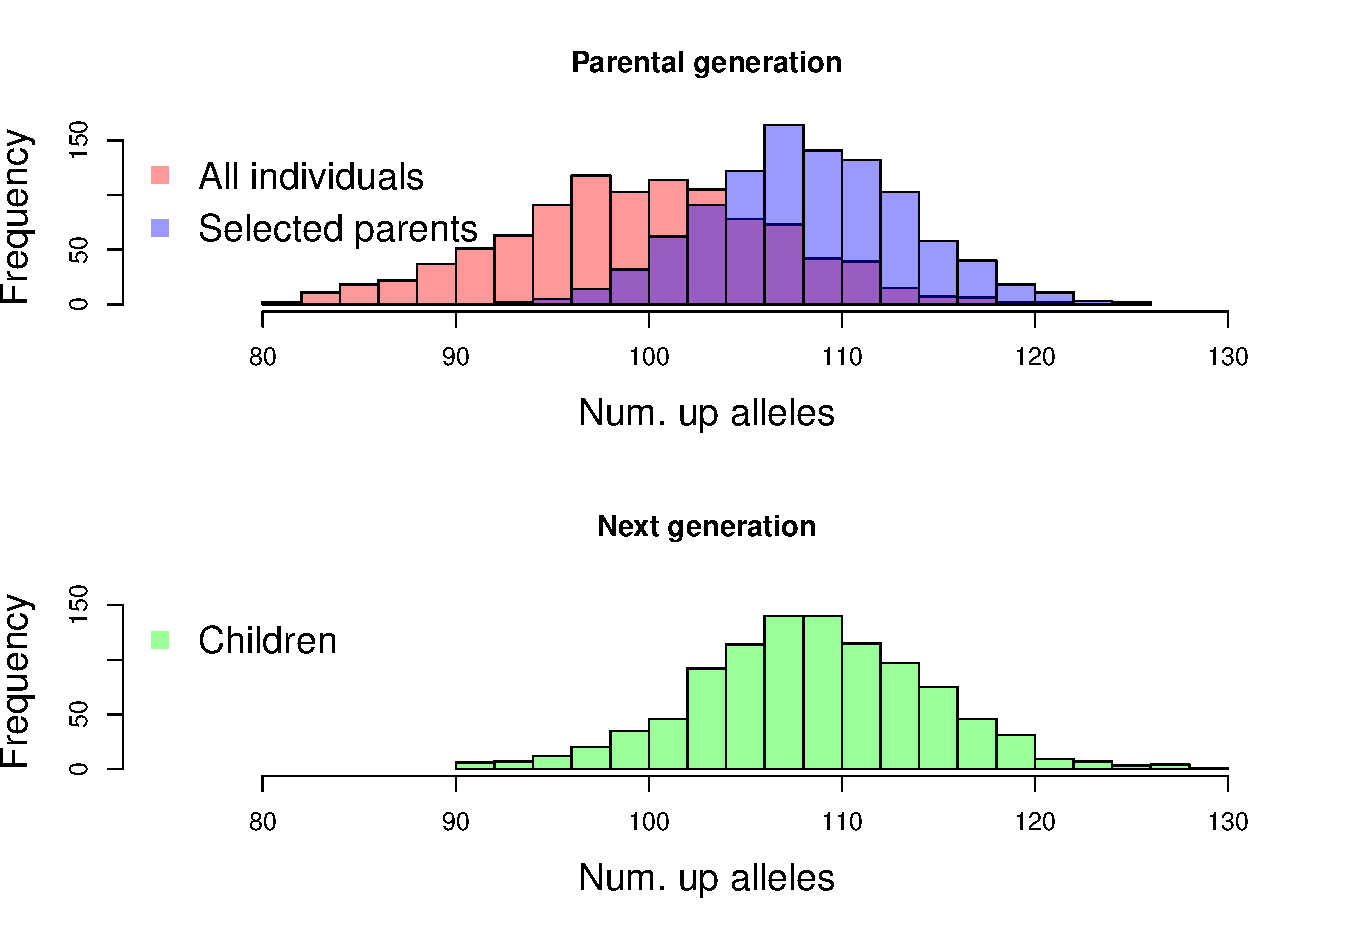
\includegraphics[width=\textwidth]{figures/QT3_w_genosums.pdf}
\end{center}
\caption[][4cm]{{\bf Top.} Distribution of the number of up alleles in the parental population
  prior to selection (red), for the selected individuals the top
  $10\%$ of the population (blue) {\bf Bottom.}  The same distribution
for the offspring of the selected parents in the next generation
(green). \gitcode{https://github.com/cooplab/popgen-notes/blob/master/Rcode/Quant_gen/QT3.R}}  \label{Fig:Response_num_alleles}
\end{figure}
 The individuals who are selected to form our next generation carry
 more alleles that increase the phenotype, in the current range of
 environments currently experienced by the population. The average
 individual before selection carried 100 of these `up' alleles, the average
 individual surviving selection 108 `up' alleles. As individuals
 faithfully transmit their alleles to the next generation the average
 child of the selected parents carries 108 up alleles. Note that the
 variance has changed little, the children have plenty of variation in
 their genotype, such that selection can readily drive evolution in future generations. The average frequency of an `up' allele has changed
 from $50\%$ to $54\%$. Gains due to selection will be stably
 inherited to future generations and can be compounded on generation
 after generation if selection pressures were to remain constant.



 \begin{marginfigure}[4cm]
 \begin{center}
   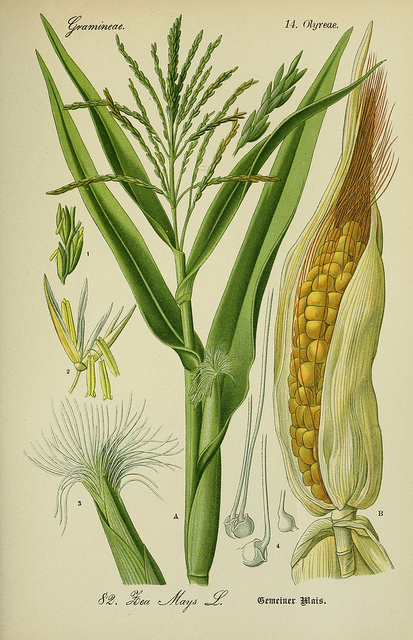
\includegraphics[width = 0.7 \textwidth]{illustration_images/Genetic_drift/maize/7845339168_66aa3d8ccc_z.jpg}
 \end{center}
 \caption{Maize ({\it Zea mays}.) \BHLNC{Prof. Dr. Thomé's Flora von
   Deutschland. 1886. Thomé, O. W.}{https://www.biodiversitylibrary.org/page/12306602\#page/669/mode/1up}{New York Botanical Garden}} \label{fig:maize}  %é
 \end{marginfigure}  %%possible different fig https://peerj.com/preprints/26502.pdf from Jeff's paper

 \paragraph{The long-term response to selection}
   \begin{marginfigure}
 \begin{center}
 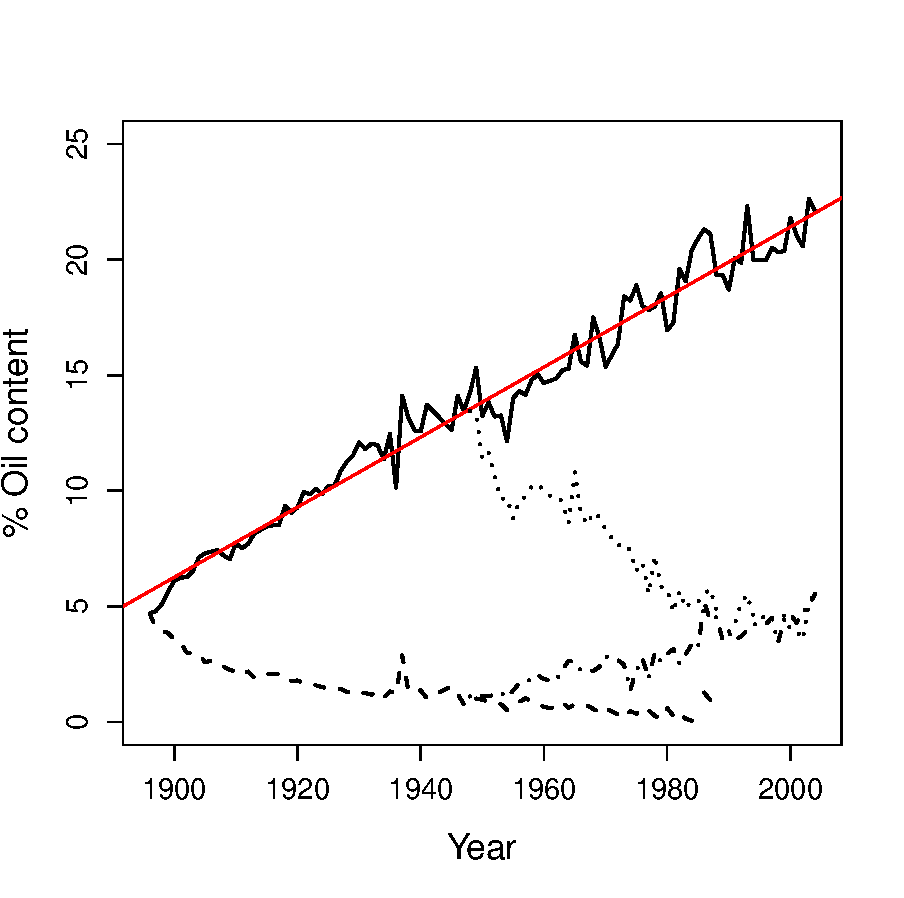
\includegraphics[width=\textwidth]{Journal_figs/Quant_gen/Illinois_long_term_selection_corn/Illinois_LTS_means.pdf} \end{center}
 \caption{The mean oil content of corn in the Illinois long term
   selection experiment. Two populations were established in 1896 from
 the same inital population. Two secondary populations were
 established in 1948 where the direction of selection was reversed.
 Linear fit to the up experiment shown as a red line. Data available \href{https://www.ideals.illinois.edu/handle/2142/3525}{here}, \gitcode{https://github.com/cooplab/popgen-notes/blob/master/Journal_figs/Quant_gen/Illinois_long_term_selection_corn/corn_LTS.R}}\label{Fig:Illinois_LTS_means}
\end{marginfigure}

If our selection pressure is sustained over many generations, we can
use our breeder's equation to predict the response. If we are willing
to assume that our heritability does not change and we maintain a constant selection
gradient, then after $n$ generations our phenotype mean will have
shifted 
\begin{equation}
n h^2 S
\end{equation}
i.e. our population will keep up a linear response to selection.
 \begin{figure}
 \begin{center}
   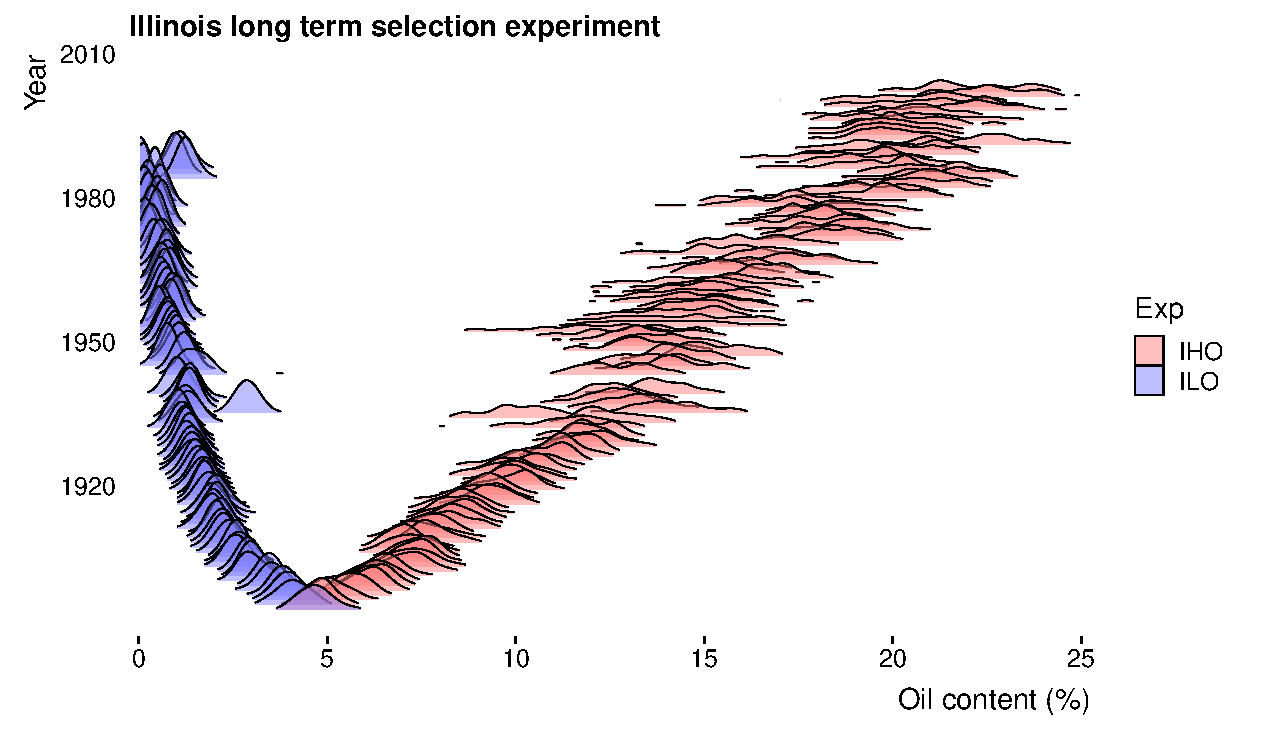
\includegraphics[width=\textwidth]{Journal_figs/Quant_gen/Illinois_long_term_selection_corn/Illinois_LTS_ggridges_distribution.pdf}\end{center}
 \caption[][2cm]{Density plots showing the phenotypic distributions of the
   up- and down-selection populations of the Illinois long term
   selection experiment over time. Data available
   \href{https://www.ideals.illinois.edu/handle/2142/3525}{here}, \gitcode{https://github.com/cooplab/popgen-notes/blob/master/Journal_figs/Quant_gen/Illinois_long_term_selection_corn/corn_LTS.R}}\label{Fig:Illinois_LTS_dists}
 \end{figure}
Therefore, long-term, consistent selection can drive impressive
evolutionary change. On example of this comes a field experiment
in Illinois, where plant breeders have systematically selected for
higher and lower oil content in corn. For over a century, they have taking seeds from the plants
in the extremes of the distribution and using them to form the next
generation. They have achieved impressive long-term responses, pushing
the population well beyond their initial range. They've established
two secondary populations where the selection differential was reversed. In the up-selection population they have maintained an
impressively linear increase in oil content (shown by red line), the
response is linear at first in the down line but they quickly reach
very low oil content.

%%single episide of selection in cliff swallows https://www.jstor.org/stable/2411315?mag=driving-evolution-cliff-swallows&seq=1#metadata_info_tab_contents
% http://mooselab.cropsci.illinois.edu/longterm.html
% https://www.ideals.illinois.edu/handle/2142/3525


\begin{question}
A population of red deer were trapped on Jersey (an island off of
England) during the last inter-glacial period. From the fossil record \cite{lister:89}
we can see that the population rapidly adapted to their new
conditions, perhaps due to selection for shorter reproductive times in
the absence of predation. Within 6,000 years they evolved from an estimated mean weight of
the population of 200kg to an estimated mean weight of 36kg (a 6 fold
reduction)! You estimate that the generation time
of red deer is 5 years and, from a current day population, that the narrow sense heritability of the
phenotype is 0.5.\\

 \begin{marginfigure}
 \begin{center}
 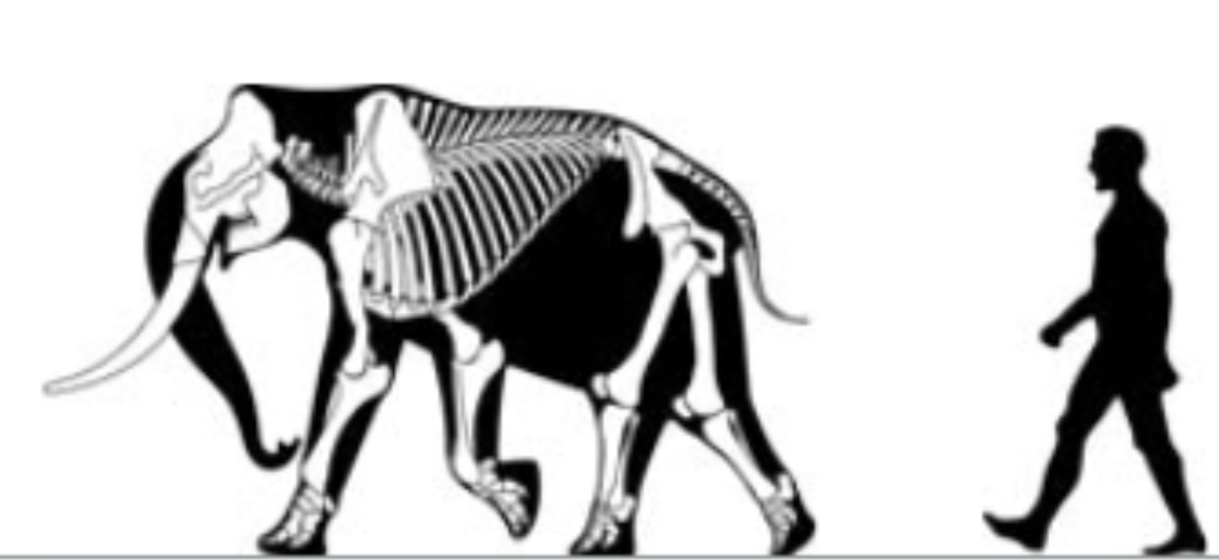
\includegraphics[width=\textwidth]{illustration_images/Quant_gen/dwarf_elephant/M_exilis_skeletal.pdf} \end{center}
 \caption{It's not just deer that evolve to be small on islands,
  pygmy mammoths and elephants have evolved from large mainland species
  on numerous islands. For example, the
   California Channel Islands were home to a dwarf mammoth until about 13,000 years
   ago. \newline \noindent \tiny{Santa
   Rosa {\it Mammuthus exilis}. \href{https://en.wikipedia.org/wiki/Pygmy_mammoth\#/media/File:M._exilis_skeletal.png}{wikimedia}, CC BY 3.0.} }\label{Fig:Pygmy_mammoth}
 \end{marginfigure}
{\bf A)}	Estimate the mean change per generation in the mean body weight. \\

{\bf B)}	Estimate the change in mean body weight caused by
selection within a generation. State your assumptions.\\

{\bf C)}	Assuming we only have fossils from the founding population and the population after 6000 years, should we assume that the calculations accurately reflect what actually occurred within our population?
\end{question}


In wild populations, selection pressures are likely rarely sustained 
for large numbers of generations. For example, the Grants' have
measured phenotypic selection in Darwin's Finches over multiple
decades on the island of Daphne Major. They have seen that
selection pressures in the Medium ground-finch ({\it Geospiza fortis})
have reversed a number of times over the years (Figure
\ref{fig:Darwins_Finches_unpred}). 

\begin{figure}
\begin{center}
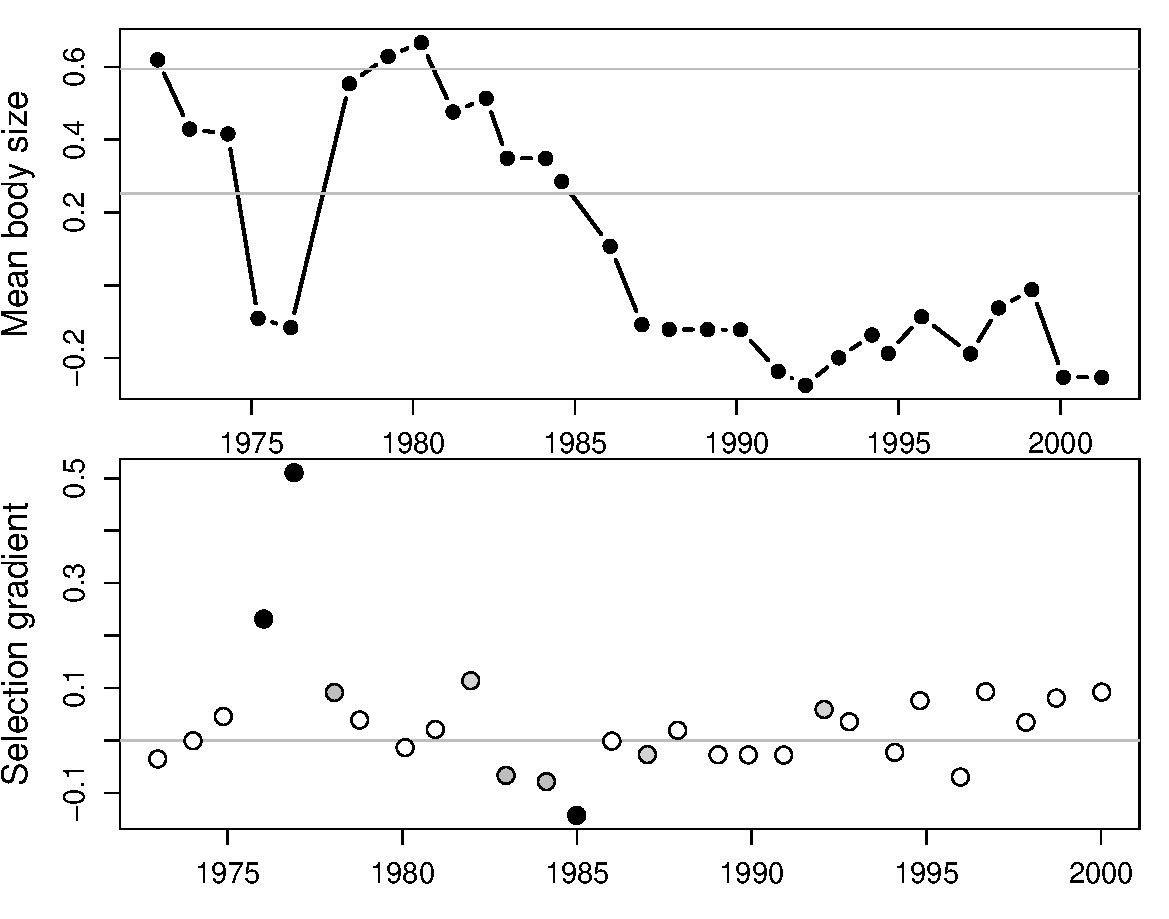
\includegraphics[width= 0.8 \textwidth]{Journal_figs/Quant_gen/Darwins_Finches_unpred/Darwins_Finches_unpred.pdf}
\end{center}
\caption[4cm]{{\bf Top)} Mean body size of the Medium ground-finch
  population measured each year, the 1973 $95\%$ confidence intervals
  are shown as horizontal bars. {\bf Bottom)} Standardized
  selection differentials on body size. The statistical significant of
  the selection differentials is shown, black points are $p<0.001$ and grey $p<0.05$.
  Data from \citet{grant2002unpredictable} \gitcode{https://github.com/cooplab/popgen-notes/blob/master/Journal_figs/Quant_gen/Darwins_Finches_unpred/Darwins_Finches_unpred.R}} \label{fig:Darwins_Finches_unpred}  
\end{figure}

\begin{marginfigure}
\begin{center}
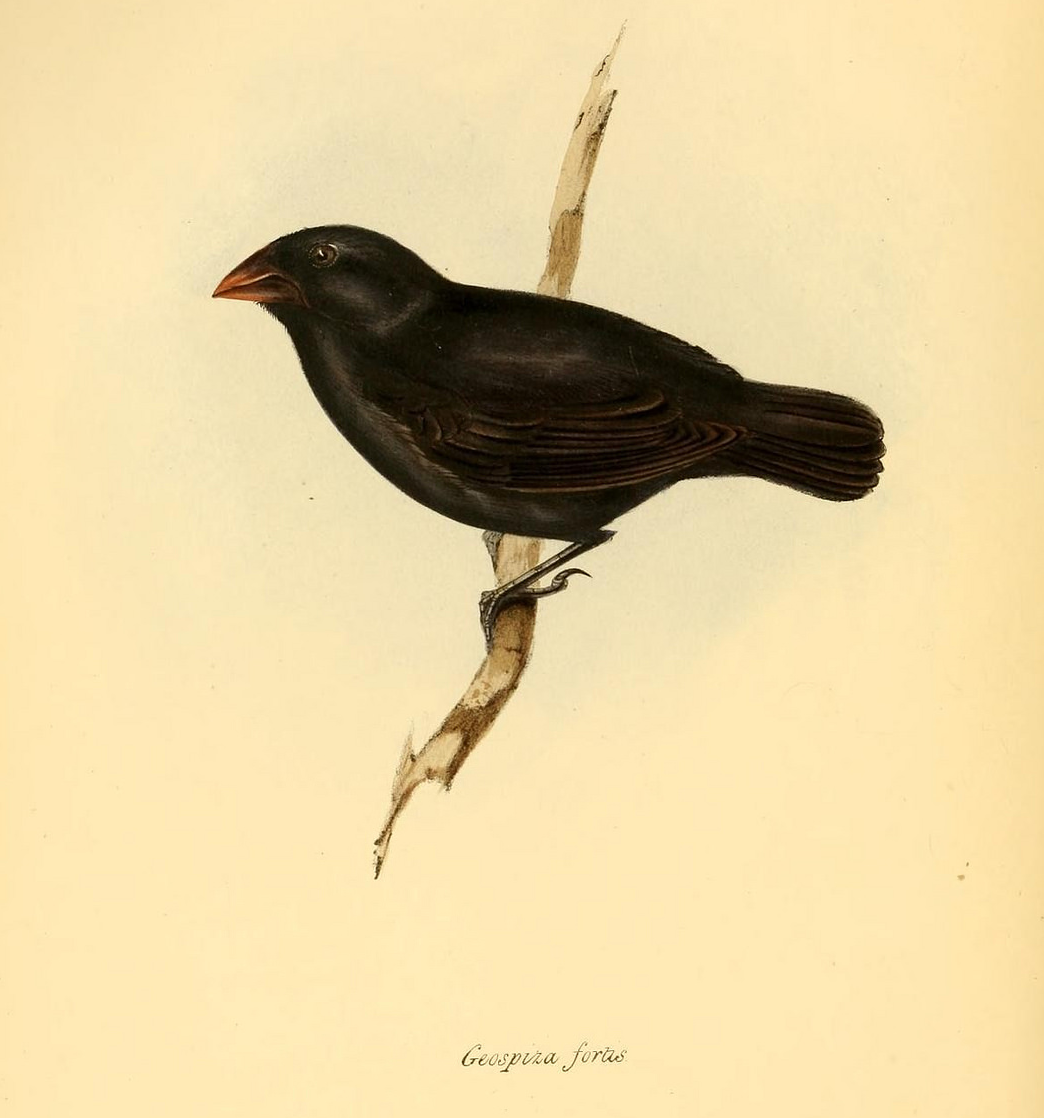
\includegraphics[width= \textwidth]{illustration_images/Quant_gen/Darwins_Finch/Geospiza_fortis.png}
\end{center}
\caption{Medium ground-finch ({\it Geospiza fortis}). \BHLNC{The zoology of
  the voyage of H.M.S. Beagle. Birds Part 3. (1841) Gould G. Edited by
  Darwin, C. Illustration by Elizabeth Gould.}{https://www.flickr.com/photos/biodivlibrary/8429528265/in/album-72157632647903291/}{Natural History Museum Library, London
}} \label{fig:Geospiza_fortis}  
\end{marginfigure}
%% Gingrich style data https://datadryad.org/resource/doi:10.5061/dryad.1tn7123?show=full
%% https://datadryad.org/resource/doi:10.5061/dryad.7d580

\section{Fitness and the Breeder's Equation.}
So directional evolution occurs as selection drives a change in
the mean phenotype within a generation. But precisely how does this relate to
the natural-selection requirement that organisms vary in their
fitness? Some different ways of formulating the Breeder's equation
give us insight into the conditions for directional selection and the
relationship to fitness landscapes.

\subsection{Directional selection as the covariance between fitness and
phenotype.}
To think more carefully about this change within a
generation, let's think about a simple fitness model where our phenotype affects the
viability of our organisms (i.e. the probability they survive to
reproduce). The probability that an individual has a phenotype $X$
before selection is $p(X)$, so that the mean phenotype before
selection is
\begin{equation}
\mu_{BS} = \E[X] =  \int_{-\infty}^{\infty} x p(x) dx
\end{equation}
The probability that an organism with a phenotype $X$ survives to
reproduce is $w(X)$, and we'll think about this as the fitness of
our organism. The probability distribution of phenotypes in those who
do survive to reproduce is
\begin{equation}
\P(X | \textrm{survive}) =  \frac{p(x) w(x)}{
\int_{-\infty}^{\infty} p(x) w(x) dx}.
\end{equation}
where the denominator is a normalization constant which ensures that
our phenotypic distribution integrates to one. The denominator also
has the interpretation of being the mean fitness of the population,
which we'll call $\wbar$, i.e.  
\begin{equation}
\wbar =  \int_{-\infty}^{\infty} p(x) w(x) dx. \label{eqn:pheno_mean_fitness}
\end{equation}
Therefore, we can write the mean phenotype in those who survive to
reproduce as
\begin{equation}
\mu_S = \frac{1}{\wbar}\int_{-\infty}^{\infty} x p(x) w(x) dx
\end{equation}
\begin{marginfigure}
  \begin{center}
    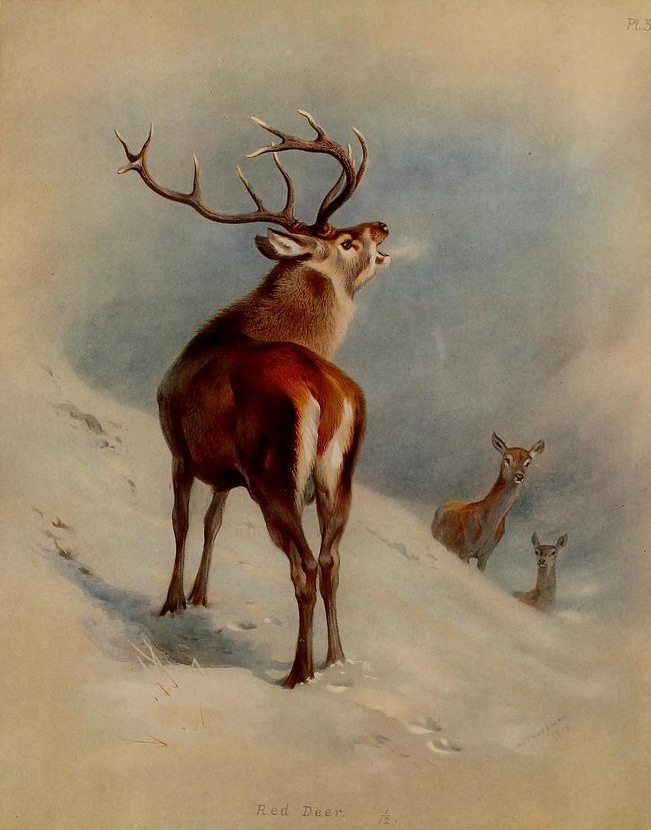
\includegraphics[width= \textwidth]{illustration_images/Quant_gen/red_deer/Red_deer.png}
\end{center}
\caption{Red deer ({\it Cervus elaphus}). \BHLCC{British
    mammals. Thorburn, A. (1920)}{https://www.flickr.com/photos/biodivlibrary/21269550204}{Field Museum of Natural History Library}{2.0}} \label{fig:red_deer}  
\end{marginfigure}

If we mean center the distribution of phenotypes in our population, i.e. set the phenotype before
selection to zero, then
\begin{equation}
S=\mu_S= \frac{1}{\wbar}\int_{-\infty}^{\infty} x p(x) w(x) dx = \E \left (X
  w(X) \right)
\end{equation}
% if $\mu_S=0$. \erin{do you mean $\mu_{BS}=0$?}
where the final part follows from the fact that the integral is taking
the mean of $X w(X)$ over the population.

As our phenotype is mean centered ($\E(X)=0$), we can see that $S$ has
the form of a covariance between our phenotype $X$ and our relative fitness
$w(X)$
\begin{equation}
  S =  \E \left (X
  w(X) \right) -\E(X)\E(w(X)) =Cov \left(X, \nicefrac{w(X)}{\wbar} \right) \label{S_covar}
\end{equation}
  Thus our change in mean phenotype is directly a measure of the
  covariance of our phenotype and our fitness. 
  Rewriting our breeder's
equation using this observation we see
\begin{equation}
R = \frac{V_A}{V}  Cov \left(X, \nicefrac{w(X)}{\wbar} \right)  
\end{equation}

we see that the response to selection is due to the fact that our
fitness (viability) of our organisms/parents covaries with our phenotype, and
that our child's phenotype is correlated with our parent's phenotype. 


\paragraph{Fitness Gradients and linear regressions}

To understand this in more detail let imagine that we calculate the
linear regression of an individual $i$'s mean-centered phenotype ($X_i$) on fitness ($W_i$), i.e. 
\begin{equation}
W_i \sim \beta X_i + \wbar \label{fitness_regression}
\end{equation}  
The best fitting slope of this regression ($\beta$), lets call it the
`fitness gradient', is given by
\begin{equation}
  \beta = Cov(X, \nicefrac{w(X)}{\wbar} )/ V  \label{beta_covar}
\end{equation}
\begin{marginfigure}
\begin{center}
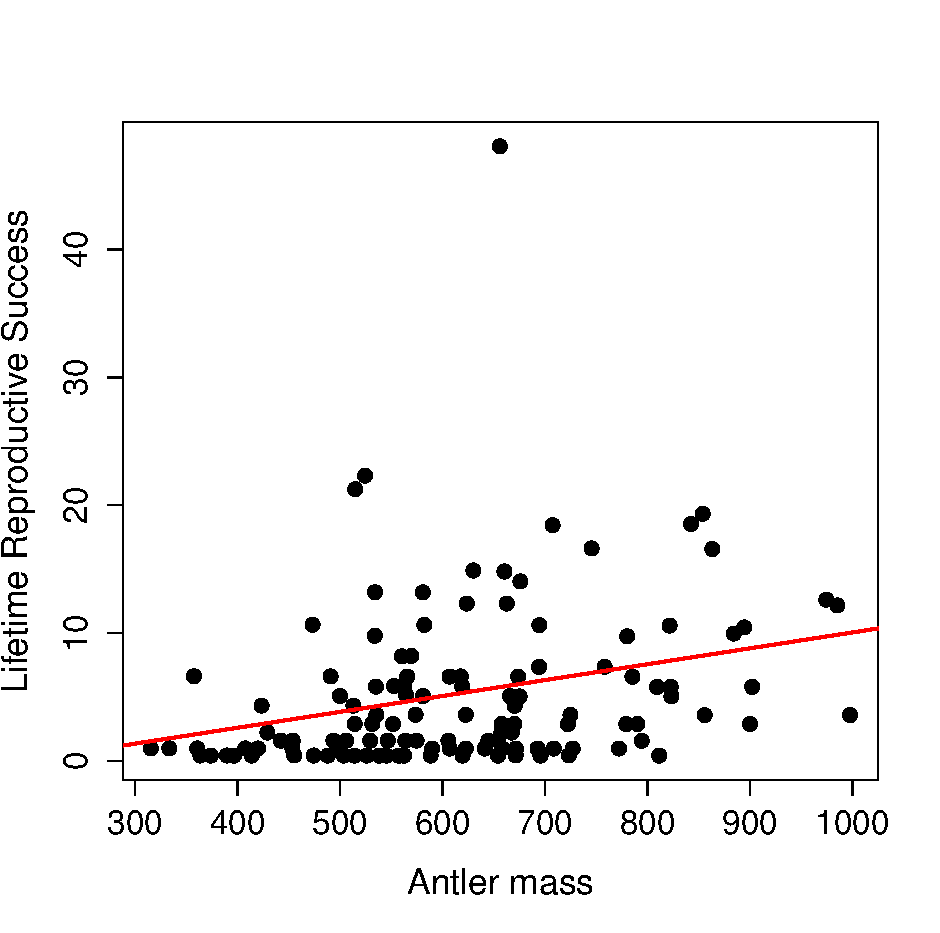
\includegraphics[width= \textwidth]{Journal_figs/Quant_gen/red_deer_selection_gradient/selection_grad_deer.pdf}
\end{center}
\caption{Lifetime reproductive success (LRS) of male Red Deer as a
  function of their antler mass. Data from \citet{kruuk2002antler},
  see the paper for discussion of the complexities of equating this
  selection gradient with the evolutionary response. \gitcode{https://github.com/cooplab/popgen-notes/blob/master/Journal_figs/Quant_gen/red_deer_selection_gradient/selection_grad_deer.R}. } \label{fig:red_deer_fitness_grad}  
\end{marginfigure}

  i.e. the fitness gradient is the covariance of phenotype-fitness
 covariance divided by the phenotypic variance. Using this result we can rewrite the breeder's equation as
\begin{equation}
R= V_A \beta \label{eqn:R_beta}
\end{equation}
i.e. we'll see a directional response to selection if there is a linear relationship of phenotype on fitness, and if there is additive genetic variance for the phenotype. As one example of a fitness gradient, in Figure \ref{fig:red_deer_fitness_grad}  the lifetime reproductive success (LRS) of male Red Deer is plotted against the weight of their antlers. The red line gives the linear regression of fitness (LRS) on antler mass and the slope of this line is the fitness gradient ($\beta$). 

\graham{add pic of relationship between slope and S?}

\paragraph{Fisher's fundamental theorem of natural selection} 
Finally how does the mean fitness of our population evolve? 
If we choose relative fitness to be our phenotype
  ($X=\nicefrac{w(X)}{\wbar}$), then the response in fitness is
\begin{align}
  R &= \frac{V_A}{V}  Cov \left(\nicefrac{w(X)}{\wbar} ,
  \nicefrac{w(X)}{\wbar} \right) = \frac{V_A}{V} V \nonumber\\
  &=V_A
\end{align}
i.e. the response to selection is equal to the additive genetic
variance for relative fitness. Or as Fisher put it
\begin{quote}
``The rate of increase in fitness of any organism at any time is equal
to its genetic variance in fitness at that time.'' -\citet{fisher1930} (pg 37)
\end{quote}
Fisher called this `the fundamental theorem of natural
selection'. Our proof here is just a sketch, and more formal
approaches are needed to show it in generality. There has been much nashing of teeth over exactly how broadly this result holds, and exactly what
Fisher meant \citep[see ][ for a recent overview]{ewens2010gene}. 
% Ruth shaw FFTNS https://www.biorxiv.org/content/biorxiv/early/2019/04/07/601682.full.pdf
% https://commons.wikimedia.org/wiki/File:A_guide_to_the_wild_flowers_(Plate_CXXV)_BHL23798491.jpg

\subsection{Directional Selection on Fitness Landscapes.}  \label{section:pheno_fitness_landscapes}

 \begin{figure*}
 \begin{center}
 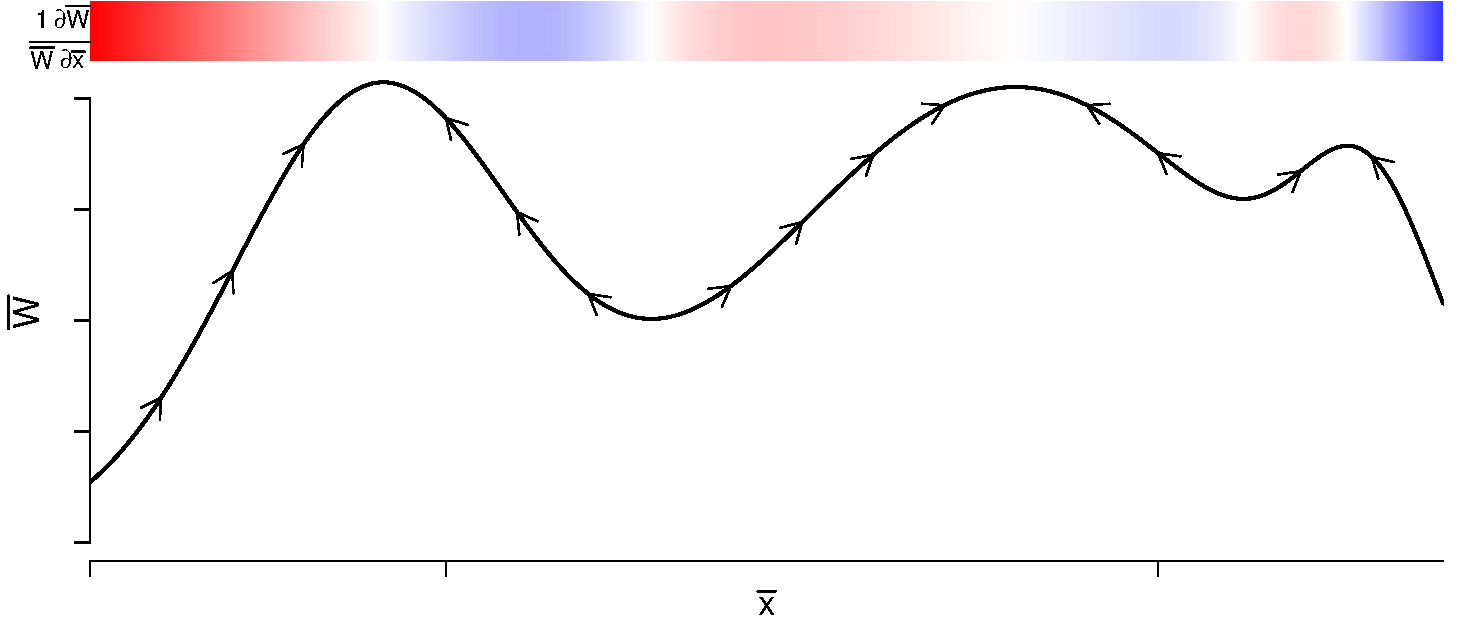
\includegraphics[width= 0.8 \textwidth]{figures/Response_to_sel/fitness_landscape_1D.pdf}
 \end{center}
 \caption{An example of a fitness landscape, showing the mean fitness
   of the population ($\wbar$) as a function of the mean phenotype of the
   population ($\bar{z}$, \gc{Need
   to change to $\bar{x}$}). The arrows show the expected direction of movement
of our population on the fitness landscape, with natural selection moving
our population toward local fitness optima. The coloured bar shows the
derivative (slope) of the mean fitness with respect to mean
phenotype (eqn. \eqref{eqn:pheno_fitness_landscape}). Red values are positive slopes corresponding to the population evolving
towards the right of the page, blue is a negative slope with the
population moving to the left. } \label{fig:fitness_landscape_1D}  
\end{figure*}

One common metaphor when we talk about evolution is that of a population exploring an adaptive landscape with natural selection pushing a population
towards higher fitness states corresponding to peaks in this landscape
(see e.g. Figure \ref{fig:fitness_landscape_1D}).  \graham{Simpson/Wright.}
\citet{lande1976natural} found an evocative formulation of the
Breeder's equation which aids our intuition of phenotypic fitness
landscapes. \graham{need note about when this breaks down}
\citeauthor{lande1976natural} showed that,
if the phenotype is
normally distributed, the response to
selection ($R$) could be written in terms of the gradient (derivative) of the
mean fitness ($\wbar$) of the population\sidenote[][3cm]{
  This follows from the fact that we can then move the
  derivative inside the integral of $\wbar$, eqn \eqref{eqn:pheno_mean_fitness}, %$\nicefrac{\partial \log\wbar}{\partial \bar{x}} = \nicefrac{1}{\wbar} \nicefrac{\partial\wbar}{\partial \bar{x}}$.
to write the new term in eqn \eqref{eqn:pheno_fitness_landscape} as 
  \begin{align}
\frac{1}{\wbar}  \frac{\partial \wbar}{\partial \bar{x}} &=
                                                                   \frac{1}{\wbar}
                                                                   \int_{-\infty}^{\infty}w(x)
                               \frac{\partial p(x)}{\partial \bar{x}}  dx \nonumber\\
& =\int_{-\infty}^{\infty} \frac{w(x)}{\wbar}  \frac{(x-\bar{x})}{V}  dx  \nonumber\\
                             & = \frac{cov(w(x),x) }{var(x)} \label{eqn:proof_landscape}
\end{align}
which is $\beta$, so that eqns \eqref{eqn:R_beta} and
\eqref{eqn:pheno_fitness_landscape} are equivalent. For this equivalence
to hold, in the first line we assume that $w(x)$ is not a function
of $\bar{x}$, while the middle line is true when $p(x)$ is the normal distribution.
}
as a function of the mean phenotype:  
\begin{equation}
  R = \frac{V_A}{\wbar} \frac{\partial \wbar}{\partial \bar{x}}  \label{eqn:pheno_fitness_landscape}  %V_A 
 % \frac{\partial \log \left(\wbar \right)}{\partial \bar{z}}
\end{equation}

What does this mean? Well $\nicefrac{V_A}{\wbar}$ is always positive,
so the direction our population responds to selection is
predicted by the sign of the derivative. If increasing the mean
phenotype of the population slightly would 
increase mean fitness ($ \nicefrac{\partial \wbar}{\partial \bar{x}}
>0$) our population will respond that generation by evolving toward
higher values of the trait ($R>0$), left panel of Figure \ref{fig:fitness_landscape_1D_w_wbar}. Conversely if decreasing the
population mean phenotype slightly would increase the mean fitness ($ \nicefrac{\partial \wbar}{\partial \bar{x}}
<0$) the population will that generation evolve towards lower values
of the phenotype, middle panel of Figure \ref{fig:fitness_landscape_1D_w_wbar}. Thus we can think of the population as evolving on
an adaptive landscape where the elevation is given by the population mean
fitness. Natural selection operates on the basis of individual-level
fitness, but as a result of this our population is increasing in its
average fitness, our population is becoming better adapted (we'll
discuss the caveats of this interpretation below).

 \begin{figure*}
 \begin{center}
 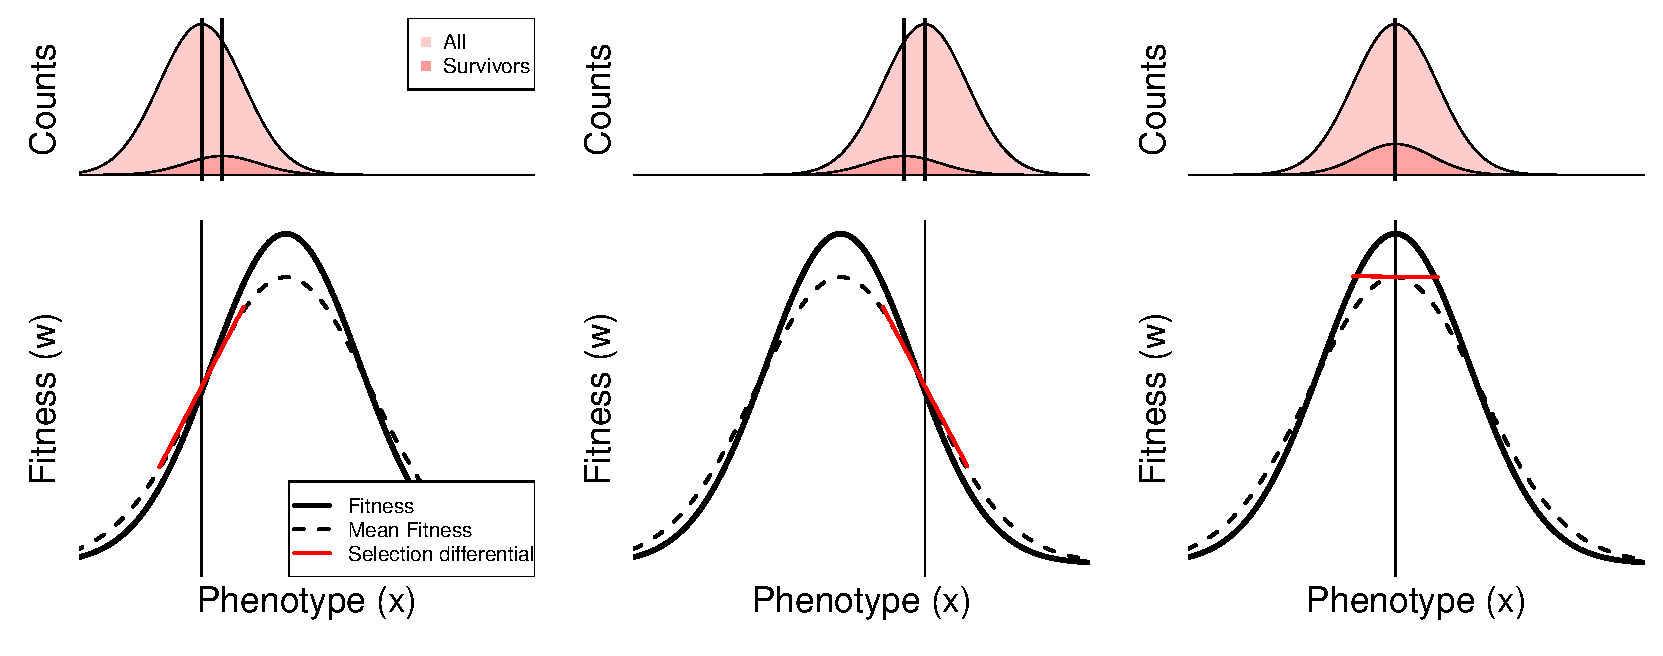
\includegraphics[width= 0.8 \textwidth]{figures/Response_to_sel/fitness_landscape_1D_w_wbar.pdf}
 \end{center}
 \caption{A population evolving on a (guassian) fitness surface. The
   bottom panel shows the expected individual fitness ($w()$) and mean
   fitess as a function of phenotype. The red line shows the best
   fitting linear approximation to the relationship between phenotype
   and fitness, eqn \eqref{fitness_regression}, whose slope is
   $\beta$. The top panel shows the distribution of the phenotype
   before and after selection. \gitcode{https://github.com/cooplab/popgen-notes/blob/master/Rcode/Quant_gen/fitness_landscape_1D_animated.R}.} \label{fig:fitness_landscape_1D_w_wbar}  
 \end{figure*}
 

What happens when it
reaches the top? Well at the top of a peak $ \nicefrac{\partial
  \wbar}{\partial \bar{x}}=0$, as it is a local maximum, and so
$R=0$. Assuming that the relationship between fitness and phenotype
stays constant, our population will stay at the top of the fitness
peak. This view of natural selection does not imply that the population
is evolving to the best possible state. Our population is just
marching up the hill of mean fitness end panel Figure
\ref{fig:fitness_landscape_1D_w_wbar}. However, this peak isn't necessarily the highest fitness peak it's just
which ever peak was closest and so our population can become trapped
on a local, but not global peak of fitness (see, for example Figure \ref{fig:fitness_landscape_1D}).

% % \animategraphics[height=2.8in,autoplay,controls]{12}{/Users/gcoop/Downloads/latex_gif/animate_gall_}{0}{14}



\begin{marginfigure}[3cm]
\begin{center}
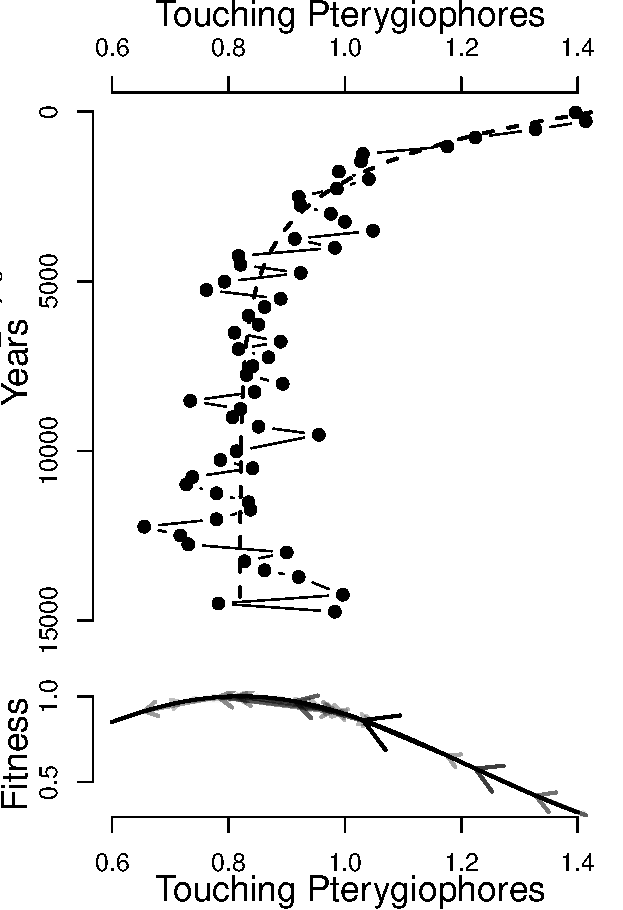
\includegraphics[width= \textwidth]{Journal_figs/Quant_gen/Stickleback_fossil_traj/Stickleback_fossil_traj.pdf}
\end{center}
\caption{{\bf Top)} A time series of stickleback phenotypic evolution from the
  fossil record. After a heavily armoured stickleback invades the lake
  it quickly evolves towards touching pterygiophores (the bones
  supporting the dorsal spines).  Fossil measurements means are
  calculated in 250 year bins. {\bf Bottom)} How our population moves
  on the Inferred fitness landscape. The arrows show each move made by
  the population in the 250 intervals. Data from
  \citet{bell2006inferring} and \citet{hunt2008evolution}  \gitcode{https://github.com/cooplab/popgen-notes/blob/master/Journal_figs/Quant_gen/Stickleback_fossil_traj/Stickleback_traj.R} } \label{fig:Stickleback_fossil_traj}  
\end{marginfigure}

One dramatical example documenting adaptive evolution to a new
fitness optimum is offered by a remarkable time-series of
stickleback evolution from a fossil lake-bed in Nevada \citep{bell2006inferring}. In this lake
the layers of sediment are laid down each year allowing a very detailed
time series with over five thousand fossils measured. The time-series
documents the evolution towards a new set of optimum phenotypes in the
fifteen thousand years after the initial invasion of the lake by a
heavily armoured stickleback species. In Figure \ref{fig:Stickleback_fossil_traj} the population mean number of
touching pterygiophores, the bones supporting the dorsal spines,
through the fossil record (Figure \ref{fig:Stickleback_fossil}). Note how quickly the species evolves toward
its new value, presumably a fitness optimum in their new environment, and the long time subsequent time interval over which
the population mean phenotype fluctuates about its new value.


\citet{hunt2008evolution} fitted a model of a population adapting to a
fitness landscape, with a single peak, to these time-series data. Their fitted fitness
surface is shown in the lower panel of Figure \ref{fig:Stickleback_fossil_traj} . The arrows show the moves that the
population mean phenotype is making on this inferred fitness
surface. The population initially takes large steps up toward the peak
of this surface and subsequently fluctuates around the peak. Under the
interpretation that there is a single stationary peak these
fluctuations represent genetic drift randomly knocking the population
offer its optimum, with selection acting to restore
the population towards this local optimum. \begin{marginfigure}
 \begin{center}
 \includegraphics[width= \textwidth]{illustration_images/Quant_gen/Fossil_stickleback/journal.pbio.1001466.g003.eps}
 \end{center}
 \caption{Fossil stickleback. Photo by Peter J. Park from \citet{losos2013evolutionary}, \PLOSccBY.} \label{fig:Stickleback_fossil}  
\end{marginfigure}

\paragraph{Issues with the Interpretation of Fitness Landscapes.}
In practice, fitness landscapes may not be constant. The environment
may be constantly changing so our population is constantly forced to run to keep
up with the fitness peak. Indeed our environment may change so quickly
that our population our population cannot keep up with the peak. Our
population is still trying to increase its mean fitness, to `adapt', but
the landscape itself is evolving.\sidenote[][1cm]{In
the case of very rapid environmental change our population may slide
further and further away the peak, and as a consequence its mean fitness
decreases which may drive the population to extinction If our
population drops below $\wbar<1$ for long enough. The conditions for
extinction are an active area of research in the field of `Evolutionary rescue'.}
More generally, for our fitness landscape result (eqn \eqref{eqn:proof_landscape}) to hold, and
for us to be able to talk of our population attempting to evolve to
higher mean fitness states,  we need the fitness of our phenotypes to be independent of the
frequency of other phenotypes in the population. (This independence allows us to
assume that the fitness of individuals is not a function of the mean
phenotype, as needed in eqn \eqref{eqn:proof_landscape}).  The
assumption of frequency independence may not hold when there is competition between individuals, e.g. for resources or
mates, as then the fitness of an individual depends on the strategies pursued
by other individuals in the populations. A classic example of this is
the fact that sexual selection may drive our
population towards pursing mate choice strategies that actively lower
the mean fitness of the population. 
% \graham{Thinking of a marble
% rolling around in the bottom of a bowl
% You could think about the
% population phenotype as a marble rolling around  }

%\paragraph{Different populations potentially sit on top of different peaks in the fitness landscape}
 % https://journals.plos.org/plosbiology/article?id=10.1371/journal.pbio.1000529

 \subsection{Stabilizing and Disruptive selection}

Up to now we have just looked at directional selection, where
selection acts to change the mean phenotype. However, we
can also use quantitative genetic models to describe other modes of
selection, extending from effects on the population mean the next
natural step is to think about selection which acts on the
population variance. Selection might act against more strongly against
individuals in the tails of the distribution, with those closer
to the mean phenotype having higher fitness, which lowers the
variance. Selection could also disfavour individuals close to the
population mean, with individuals with extreme phenotypes having
higher fitness, which acts to increase the fitness. 

Directional selection occurs because of the covariance
between our phenotype and fitness, eqn \eqref{S_covar}. Just as we expressing directional selection as a covariance allowed us to
characterize directional selection as the linear relationship between
fitness and and phenotype, $\beta$, we can summarize the variance
reducing selection by including a quadratic term in the regression of
fitness on phenotype
\begin{equation}
w_i \sim \beta x_i + \nicefrac{1}{2}  \gamma x_i^2  + \wbar \label{fitness_regression_stab}
\end{equation}
This $\gamma$, the coefficient of the quadratic term in our model, is the
quadratic selection gradient: the covariance of fitness and the squared
deviation from the phenotypic mean ($\mu_{BS}$), i.e.
\begin{equation}
\gamma = \frac{Cov\left(w(X), (X-\mu_{BS})^2 \right)}{V^2}
\end{equation}
Our $\gamma$ describes the curvature of the fitness surface around the
mean. \marginnote[-1.5cm]{Just like how $\beta$ could be interpreted
as the mean gradient of the fitness surface, our $\gamma$ is the
mean curvature of the fitness surface
  \begin{equation}
\gamma = \E \left[\nicefrac{\partial^2 w(x)}{\partial x^2}  \right] =
\int \nicefrac{\partial^2 w(x)}{\partial x^2} p(x) dx
\end{equation}
\graham{Need to straighten out issues with mean fitness vs fitness in
  these sections}
}
Values of $\gamma<0$  are consistent with stabilizing selection,
reducing the variance. While values of $\gamma>0$ are consistent with disruptive
selection, increasing the variance. \graham{add refs about this not being sufficient}

%To do this we can think about how selection acts 

% https://onlinelibrary.wiley.com/doi/pdf/10.1111/j.1469-1809.1951.tb02469.x

\begin{figure}
\begin{center}
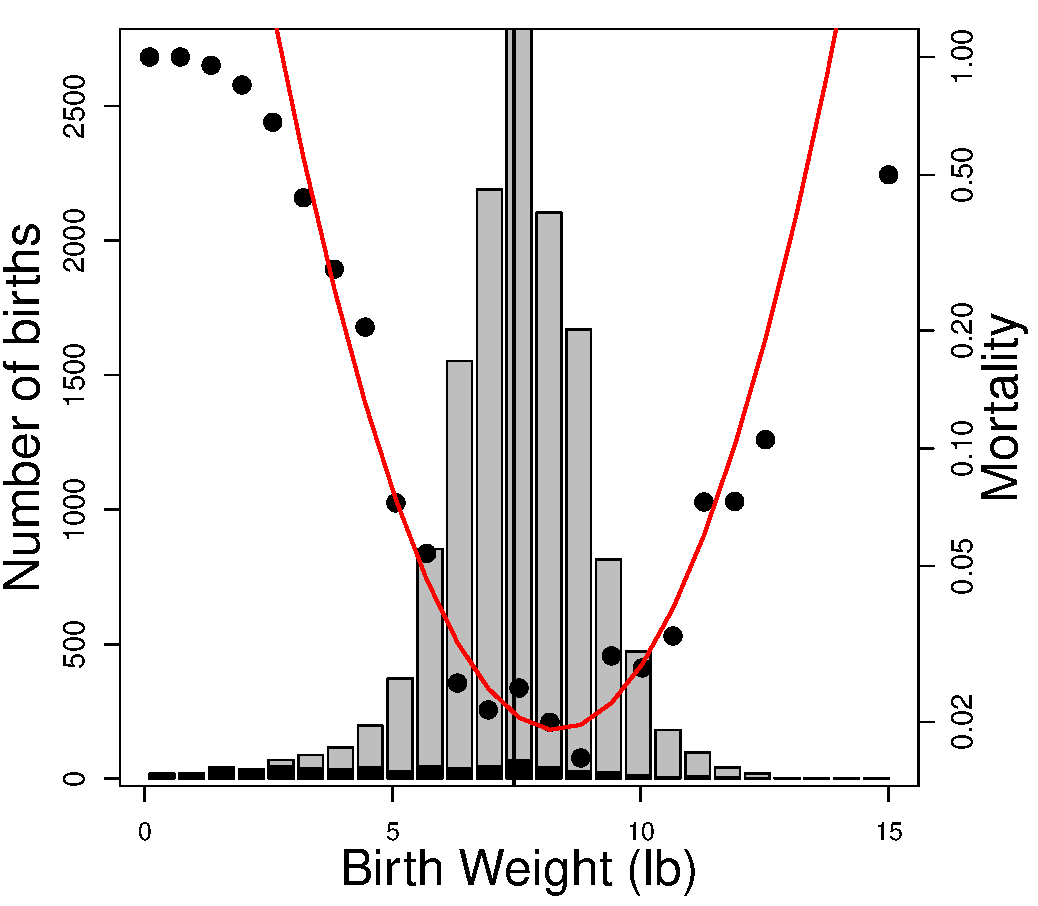
\includegraphics[width= 0.6 \textwidth]{Journal_figs/Quant_gen/birth_weight/Karn_Penrose_birth_weight.pdf}
\end{center}
\caption{Bars show the total number of births with different birth
  weights (left axis)  Dots show the mortality probability for different
  birth-weight bins (right axis), the red line shows a fitted
  quadratic model to mortality. Data from \citet{karn1951birth}
  Table 2, collapsing male and female births, \gitcode{https://github.com/cooplab/popgen-notes/blob/master/Journal_figs/Quant_gen/birth_weight/birth_weight_selection.R} } \label{fig:Birth_weight}  
\end{figure}

Under stabilizing selection the individuals with extreme phenotypes in
either tail have lower fitness, the result of which is to reduce the
phenotypic variance within a generation. A classic case of stabilizing selection
is birth weight in humans \citep{karn1951birth}. Mary Karn collected
data for nearly fourteen thousand pregnancies from 1935-46 for birth
weight and mortality. These data are replotted in Figure
\ref{fig:Birth_weight}. The variance of all births is $1.575$lb$^2$, while in live births this
was reduced to $1.26$lb$^2$, a 20\% reduction in variance due to
stabilizing selection. It is worth noting, that this selection
pressure has been greatly reduced over the decades in societies with
access to good prenatal care \citep{ulizzi1992natural}.  %, a large effect of which has been to
%reduce the variance in birth weights due to better nutrition

%womb https://www.google.com/search?q=leonardo+da+vinci+baby&tbm=isch&source=iu&ictx=1&fir=pl1GYGee8iN0gM%253A%252CEdMTKcL8foK_hM%252C_&vet=1&usg=AI4_-kRCaAAUfKDX5AEtEm6lUZ5hjWMPlw&sa=X&ved=2ahUKEwjkluyapsniAhVWs54KHX7GBFsQ9QEwA3oECAMQCg#imgrc=W3ZPdyKQE9YkRM:&vet=1

\begin{marginfigure}
\begin{center}
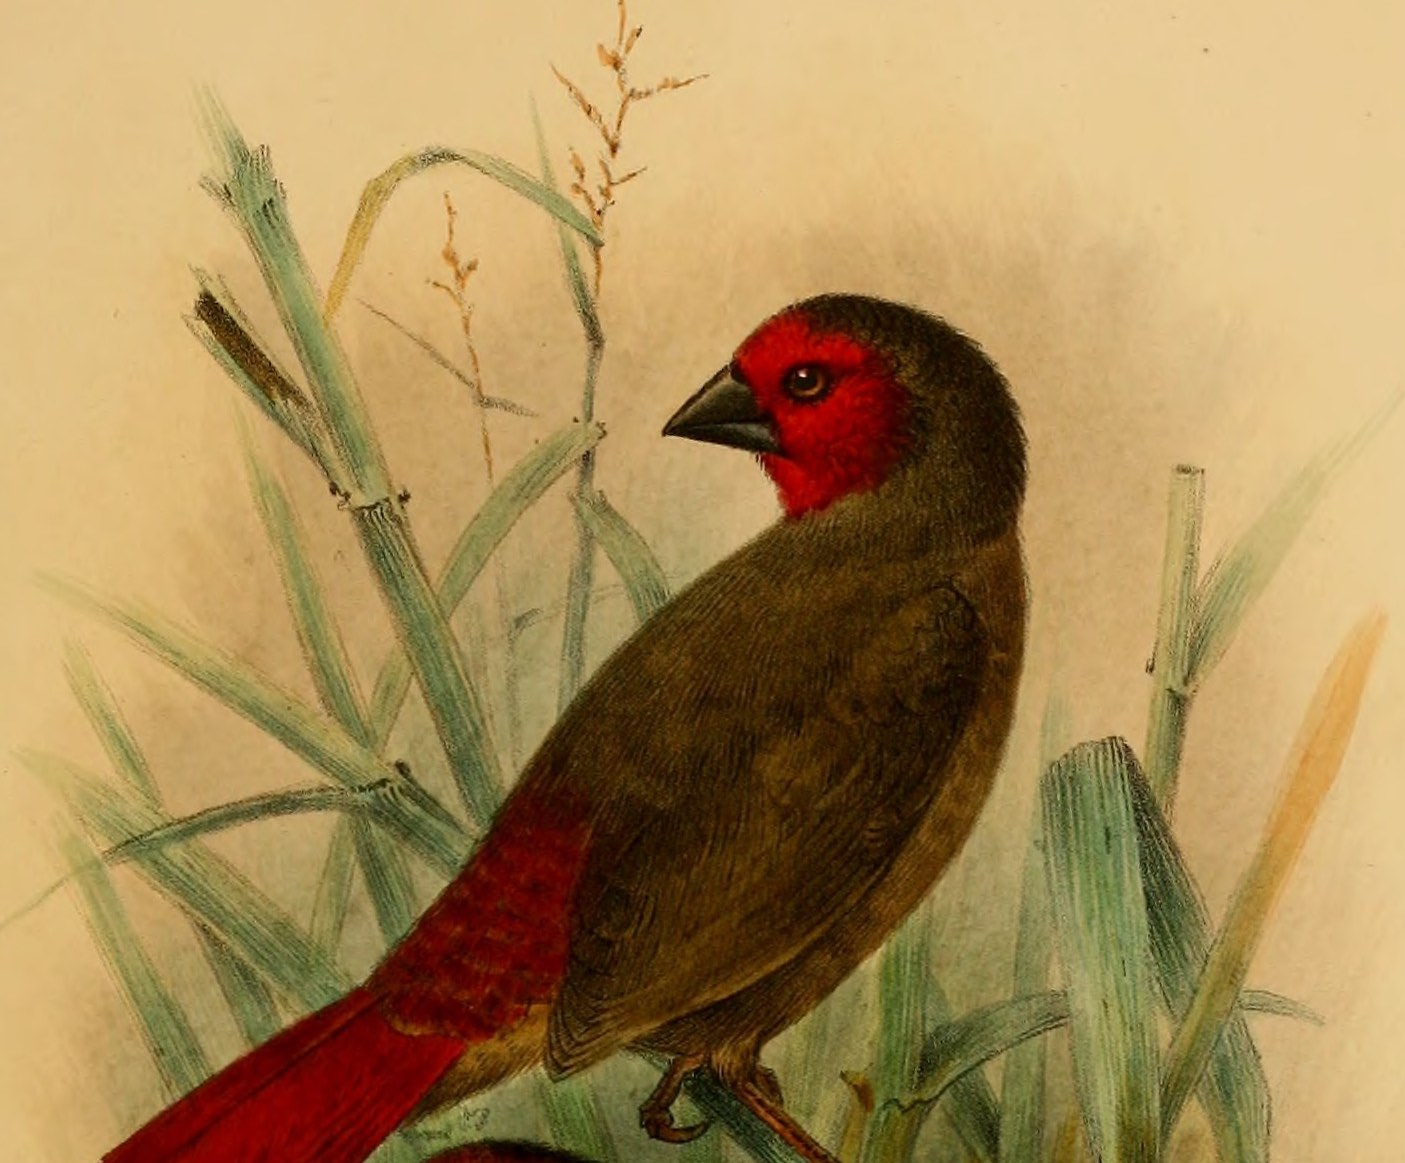
\includegraphics[width= \textwidth]{illustration_images/Quant_gen/Pyrenestes_seedcracker/Pyrenestes_minor.jpg}
\end{center}
\caption{Lesser seedcracker {\it Pyrenestes minor} a close relative of
  the Black-bellied seedcracker, whose beak is about the same size as
  the smallest Black-bellied individuals. \BHLNC{The birds of Africa, comprising all the species
    which occur in the Ethiopian region. (1986) Sclater, W. L Plate by  H. Gr{\"o}nvold}{https://archive.org/stream/birdsofafricacom41shel/birdsofafricacom41shel\#page/n306/mode/1up}{Smithsonian Libraries} }  
\end{marginfigure}
In Central Africa, Black-bellied seedcrackers ({\it
  P. ostrinus}) show disruptive selection on a remarkable beak-size polymorphism (Figure \ref{Black_bellied_seedcrackers_beaks}).  The small-beaked individuals feed on
soft  seeds from one species of marsh sedge while the big-beaked
individuals feed on hard seeds from another sedge, which
requires ten times the force to crack.  \citet{smith1993disruptive}
recorded the fates of hundreds of juveniles, and found that
individuals with intermediate beak sizes survived at much lower rates,
Figure \ref{Black_bellied_seedcrackers_beaks}, because they were not
well adapted to either seed resource.  Break length is subject to
disruptive selection, as can also be seen by the significant negative quadratic
term in the regression of survival probability on break length. The variance of mandible in the total sample of individuals was
$0.5$mm$^2$ in the survivors this variance increased by a factor of
almost $\times 2.5$ to $1.3$mm$^2$.  

\begin{figure}
\begin{center}
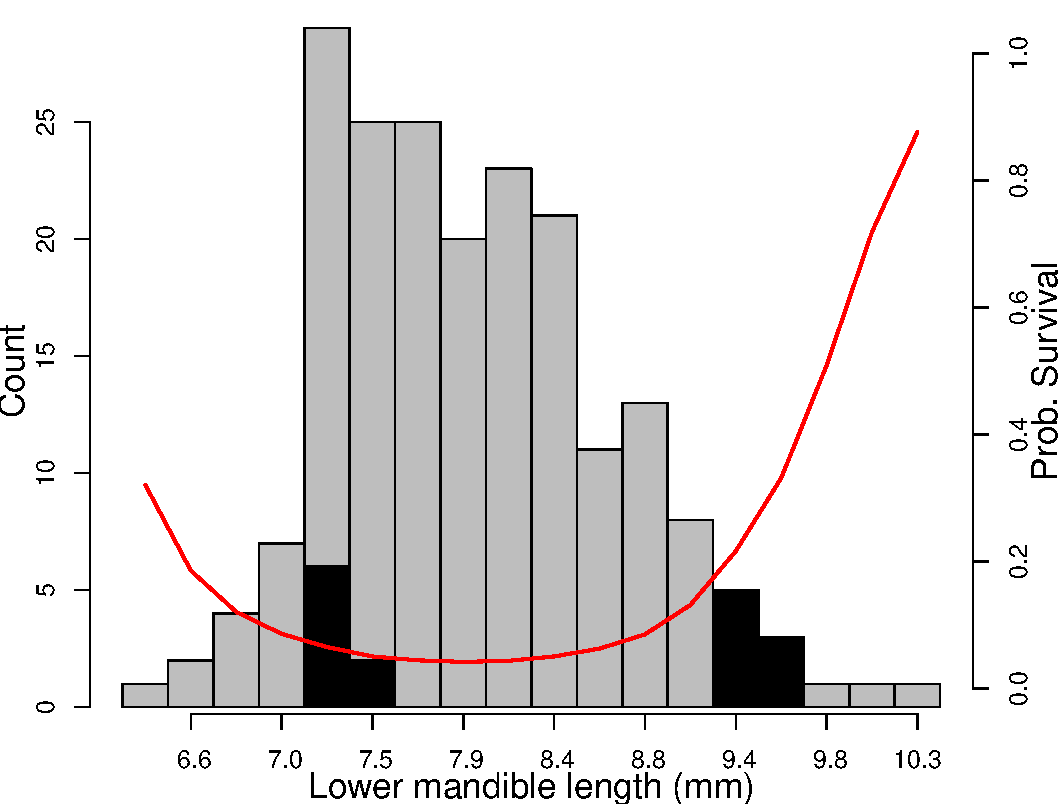
\includegraphics[width= \textwidth]{Journal_figs/Quant_gen/Smith_black_bellied_seed_cracker/Smith_black_bellied.pdf}
\end{center}
\caption{ {\bf Left} An illustration of the the remarkable variation
  in beak size within Black-bellied seedcrackers ({\it  P.
    ostrinus}). {\bf Right} A histogram of a beak size measurement in
  Black-bellied seedcrackers, all juveniles are shown in white, while the
  black bars show the survivors. The red curve shows the best fitting
  linear and quadratic model to the probability of survival, fitted
  using a binomial generalized linear models with a logit link function.  
  \BHLNC{Left illustration from: Size variation in {\it Pyrenestes} by
    Chapin J.P. in the Bulletin of the
    American Museum of Natural History (Vol. XLIX
    1923)}{https://archive.org/stream/bulletinofameric49alleuoft/\#page/417/mode/1up}{Toronto
    Library}   } \label{Black_bellied_seedcrackers_beaks}
\end{figure}


To illustrate how directional selection and quadratic terms play off
during adaptation, lets consider the goldenrod gall fly ({\it Eurosta solidaginis}), aka the goldenrod
ball gallmaker. See Figure \ref{gall_size_stab}. As it's wonderful name
implies this insect lays its eggs in Goldenrod plants, and the larvae
release chemicals forcing the plant to form a gall that forms a home
for the larvae as they develop. While this seems like a pretty sweet
deal for the larvae, it is not without its perils. \begin{marginfigure}[2cm]
\begin{center}
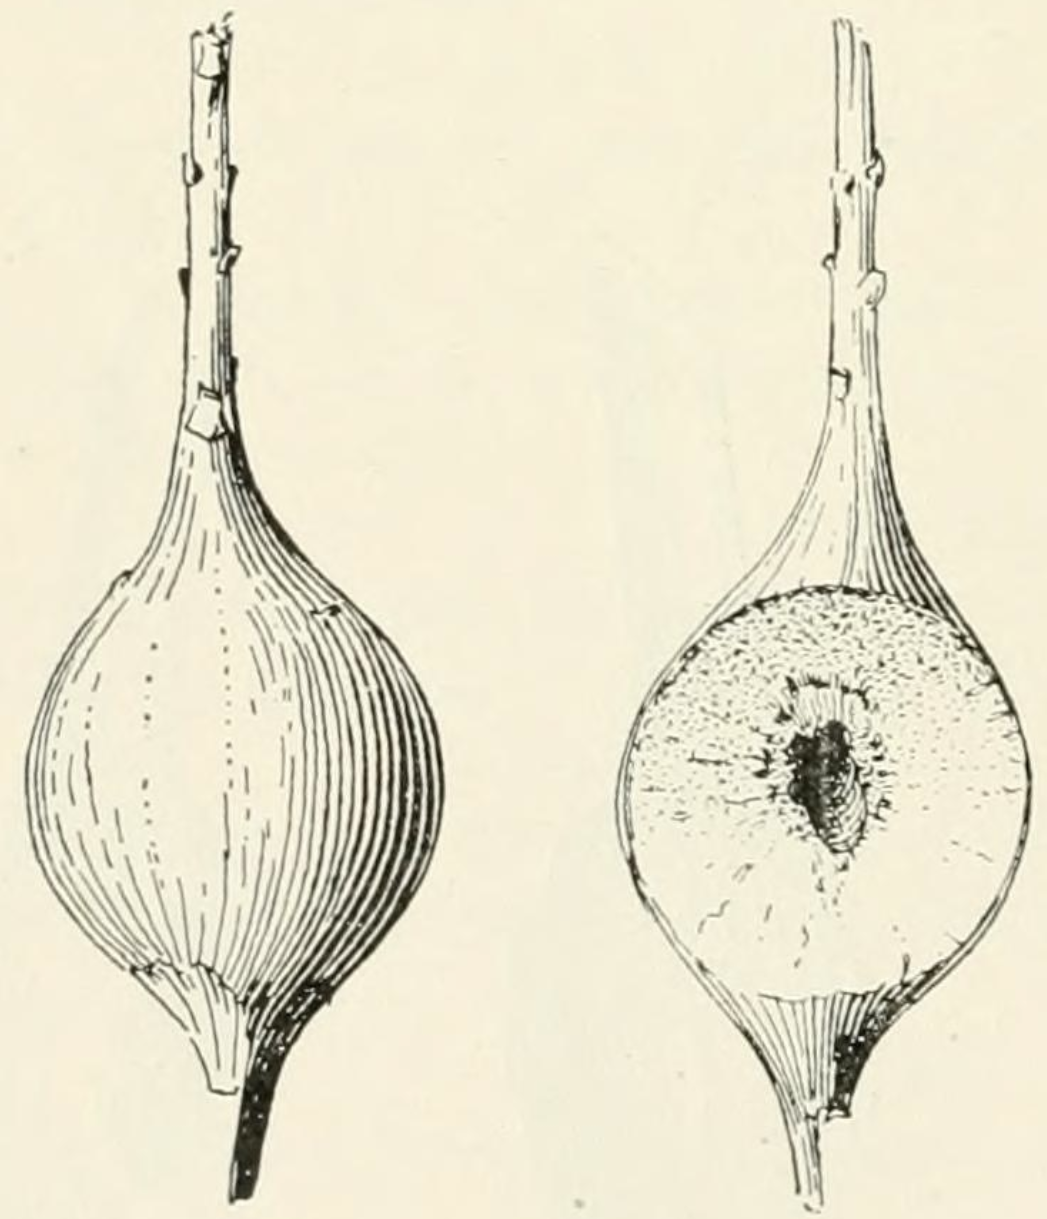
\includegraphics[width= 0.7 \textwidth]{illustration_images/Quant_gen/goldenrod_ball_gall_maker/goldenrod_ball_gall_maker.png}
\end{center}
\caption{The gall formed by the goldenrod
ball gallmaker ({\it Eurosta solidaginis}) in a goldenrod plant. The
one on the right is cut to show a partial cross-section. \BHLNC{Annual report of the New York State Museum (1917)}{https://archive.org/stream/annualreport71newy/\#page/196/mode/1upp}{The LuEsther T Mertz Library, the New York Botanical Garden} }  
\end{marginfigure}
When the small, ball galls fall risk of parasitism from parasitoid
wasps. This selection drives strong positive directional selection on
gall size, with little stabilizing selection, notice that the good
agreement between the linear selection gradient and the fit including
a linear and quadratic term. However, bigger galls fall under the pall of predation from downy
woodpeckers and black-capped chickadees, who seek out the tasty
larvae. Thus intermediate size galls are favoured, a fitness peak that
the population quickly reaches this fitness peak. Once on this peak,
there is no directional selection, i.e. no linear slope, but there
is strong stabilizing selection, i.e. a quadratic term. 

\begin{figure}
\begin{center}
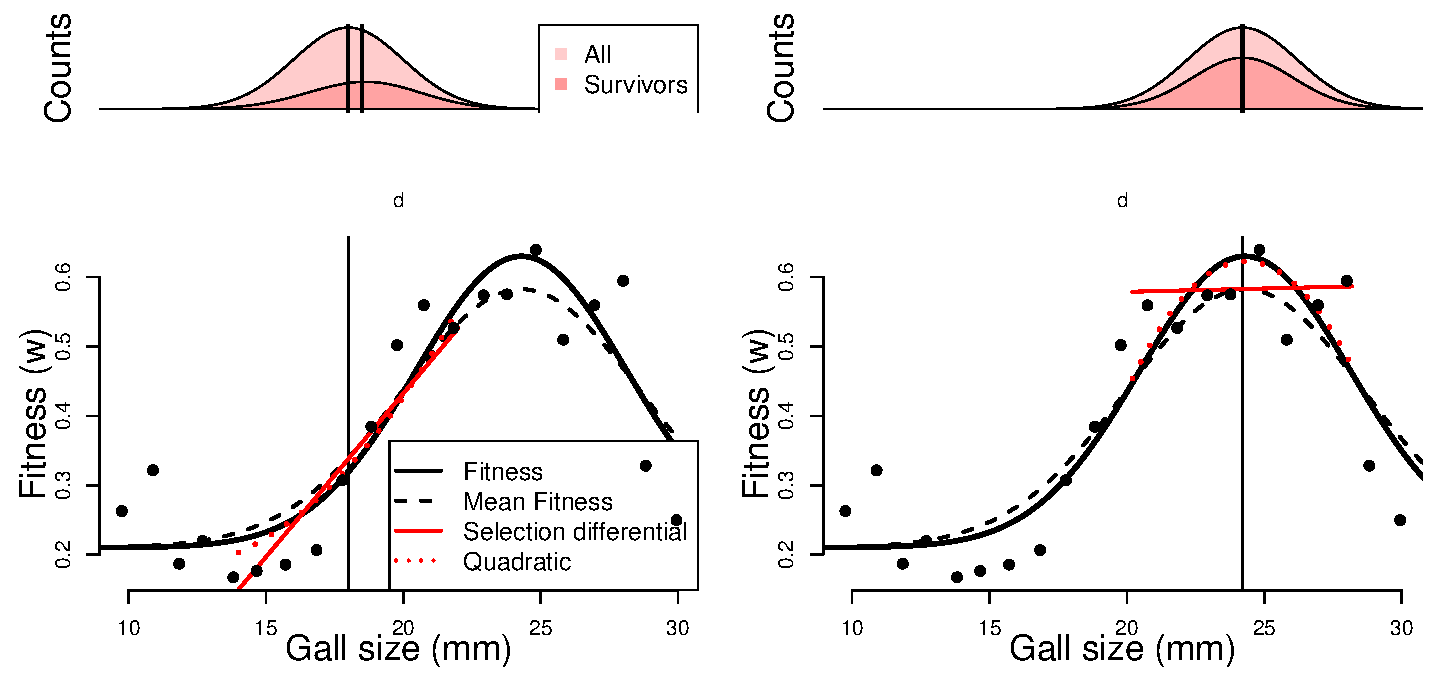
\includegraphics[width= \textwidth]{Journal_figs/Quant_gen/Weis_Gorman_gall_size_stablizing_sel/gall_size.pdf}
\end{center}
\caption[2cm]{Fitness surface for gall diameter in goldenrod
ball gallmakers. The dots are the measured survival probabilities of
bins of different sized galls.The solid line is a fitted individual fitness
  surface ($w(~)$). Dotted line is $\wbar$ plotted as a function of
  the population mean assuming a normal distribution with a standard
  deviation of $2$mm. Data from \citet{weis1990measuring}, \gitcode{https://github.com/cooplab/popgen-notes/blob/master/Journal_figs/Quant_gen/Weis_Gorman_gall_size_stablizing_sel/gall_size_fitness_landscape.R}} \label{gall_size_stab}
\end{figure}


%%% selection on gall size https://sci-hub.tw/https://onlinelibrary.wiley.com/doi/abs/10.1111/j.1558-5646.1990.tb03807.x
% https://www.flickr.com/photos/internetarchivebookimages/18429735991/
%https://archive.org/stream/annualreport71newy/#page/196/mode/1up


%black beelied seed cracker
%https://sci-hub.tw/https://www.nature.com/articles/363618a0
%https://www.flickr.com/photos/internetarchivebookimages/20416920856/in/photolist-otagrj-xVVxst-wRSxF1-x7b4fQ-x9uxzB
%https://www.flickr.com/photos/internetarchivebookimages/14755609045/
 
% Cross bill https://www.google.com/search?q=loxia+curvirostra+biodiversity+heritage+library&source=lnms&tbm=isch&sa=X&ved=0ahUKEwjItfbRm87iAhUyMn0KHZDNDlIQ_AUIECgB&biw=1440&bih=726#imgrc=cfi-GvhZRX1zxM:
% https://sci-hub.tw/https://www.jstor.org/stable/2937103?seq=1#metadata_info_tab_contents


%file:///Users/gcoop/Downloads/calsbeek2008.pdf  disruptive selection
%on leg length in anoles
 

\section{The response of multiple traits to selection.}
We can generalize these results for multiple traits, to ask how selection on
multiple phenotypes plays out over short time intervals. \cite{lande:79} Considering two traits we can write our responses in both traits as
\begin{eqnarray}
R_1 & = V_{A,1} \beta_1 + V_{A,1,2} \beta_2 \nonumber \\
R_2 & = V_{A,2} \beta_2 + V_{A,1,2} \beta_1  \nonumber \\
\end{eqnarray}
where the $1$ and $2$ index our two different traits. Here $V_{A,1,2}$ is our additive covariance between our traits. Our selection gradient for trait 1, $\beta_1$, represents the change in fitness changing trait 1 alone holding everything else constant. This is a statement that our response in any one phenotype is modified by selection on other traits that covary with that trait. This offers a good way to think about how genetic trade offs play out over short-term evolution.

We can also write this in matrix form. We can write
our change in the mean of our multiple phenotypes within a generation as the vector $\bf{S}$ and our response across multiple generations as
the vector $\bf{R}$. These two quantities are related by 
\begin{equation}
\bf{R} = \bf{G} \bf{V}^{-1} \bf{S} = \bf{G} \boldsymbol{ \beta}
\end{equation}
 where $\bf{V}$ and $\bf{G}$ are our matrices of the
 variance-covariance of phenotypes and additive genetic values
 (eqn. \eqref{G_matrix} \eqref{P_matrix}) and
 $\boldsymbol{\beta}$ is a vector of selection gradients (i.e. the change within a generation as a fraction of the total phenotypic variance). 

\gc{Need to add example of using this.}
 
\begin{question}
You collect observations of red deer within a generation, recording an
individual's number of offspring and phenotypes for a number of traits which are known to
have additive genetic variation. Using your data, you construct the plots shown in
Figure \ref{fig:red_deer_Q} (standardizing the phenotypes). Answer the following
questions by choosing one of the bold options. Briefly justify each of your answers with reference to the breeder's
equation and multi-trait breeder's equation. \\
{\bf A)}	Looking just at figure \ref{fig:red_deer_Q} A, in what direction do you expect male antler size to evolve? \\
{\bf Insufficient information, increase, decrease.}\\

{\bf B)}	Looking just at figures \ref{fig:red_deer_Q} B and C, in what direction do you expect male antler size to evolve? \\
{\bf Insufficient information, increase, decrease.}\\

{\bf C)}	Looking at figures \ref{fig:red_deer_Q} A, B, and C, in what direction do you expect male antler size to evolve? \\
{\bf Insufficient information, increase, decrease.}\\
\end{question}


\begin{figure}
\begin{center}
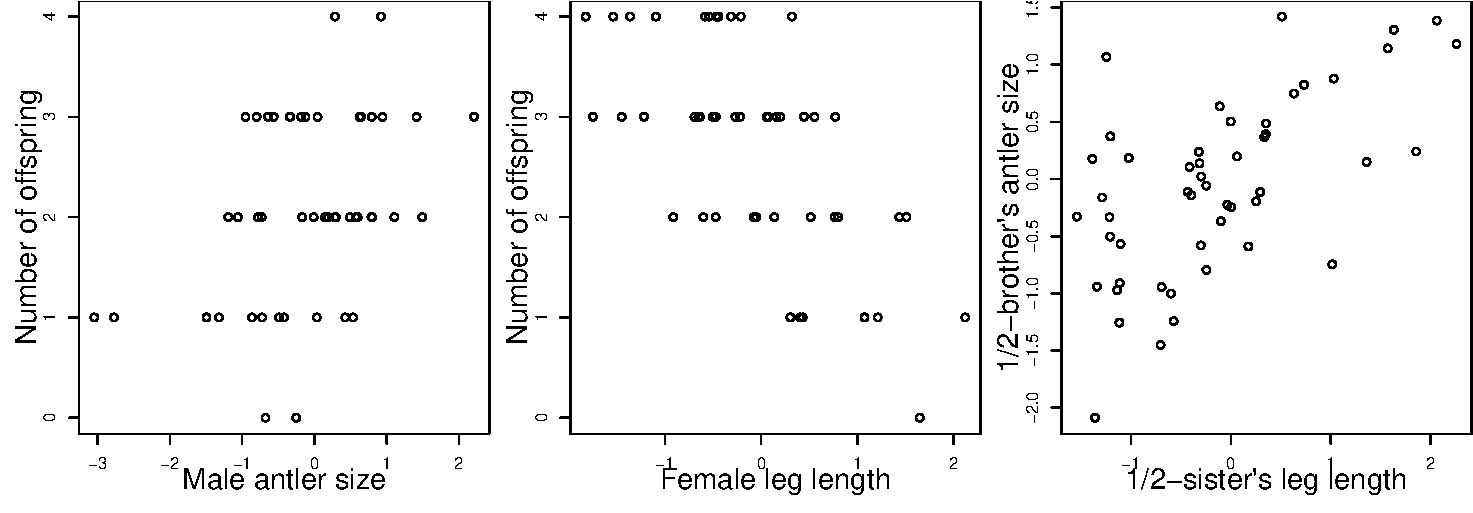
\includegraphics[width=\textwidth]{figures/Red_deer_selection.pdf}
\end{center}
\caption{ Observations of red deer within a generation; recording an
individual's number of offspring and phenotypes (simulated data), which are known to
have additive genetic variation. The figures left to right are
A-C. (Data are simulated. \gitcode{https://github.com/cooplab/popgen-notes/blob/master/Rcode/Red_deer_MV_selection.R}) } \label{fig:red_deer_Q}
\end{figure}


As an example of correlated responses to selection, consider the  \citet{wilkinson:93} selection experiment on Stalk-eyed
 flies ({\it Cyrtodiopsis  dalmanni}). Stalk-eyed flies have evolved amazingly long eye-stalks. In the lab, \citeauthor{wilkinson:93} established six populations of
 wild-caught flies and selected up and down on males eye-stalk to body
 size ratio for 10 generations (left plot in Figure
 \ref{fig:Stalk_eyed_response}). Despite the fact that he did not
 select on females, he saw a correlated response in the females from
 each of the lines (right plot), because of the genetic correlation
 between male and female body proportions. 

\begin{figure}
\begin{center}
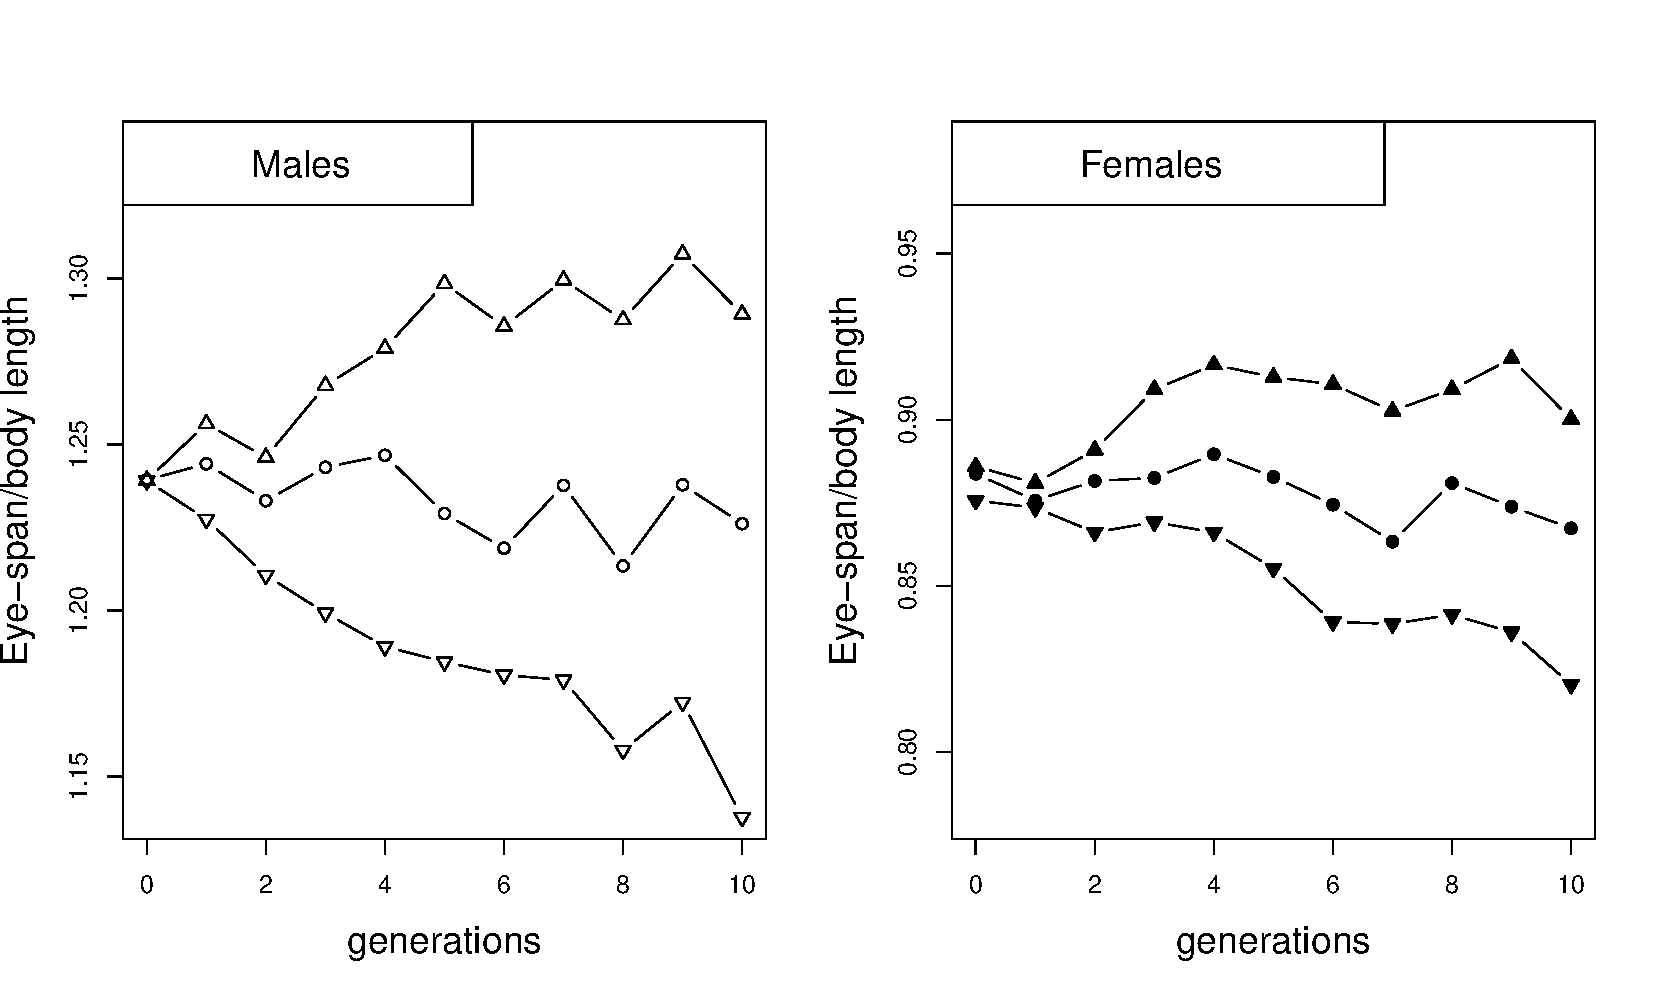
\includegraphics[width= \textwidth]{Journal_figs/Quant_gen/stalk_eyed_flies/stalk_eyed_flies_response.pdf}
\end{center}
\caption[][-2cm]{ \citeauthor{wilkinson:93} selected two of populations for flies for
 increased and eye-stalk to body length ratio in males (mean shown as
 up triangles), and two for a
 decreased ratio (down triangles), by taking the top 10 males with the highest (lowest)
 ratio out of 50 measures. He also established two control populations
 (circles). He constructed each generation of females by sampling 10
 at random from each population.  Data from \citet{wilkinson:93}. \gitcode{https://github.com/cooplab/popgen-notes/blob/master/Journal_figs/Quant_gen/stalk_eyed_flies/Wilkinson_93_response_to_sel.R} } \label{fig:Stalk_eyed_response}   %\cite{potti:11} 
\end{figure}

\begin{marginfigure}[1cm]
\begin{center}
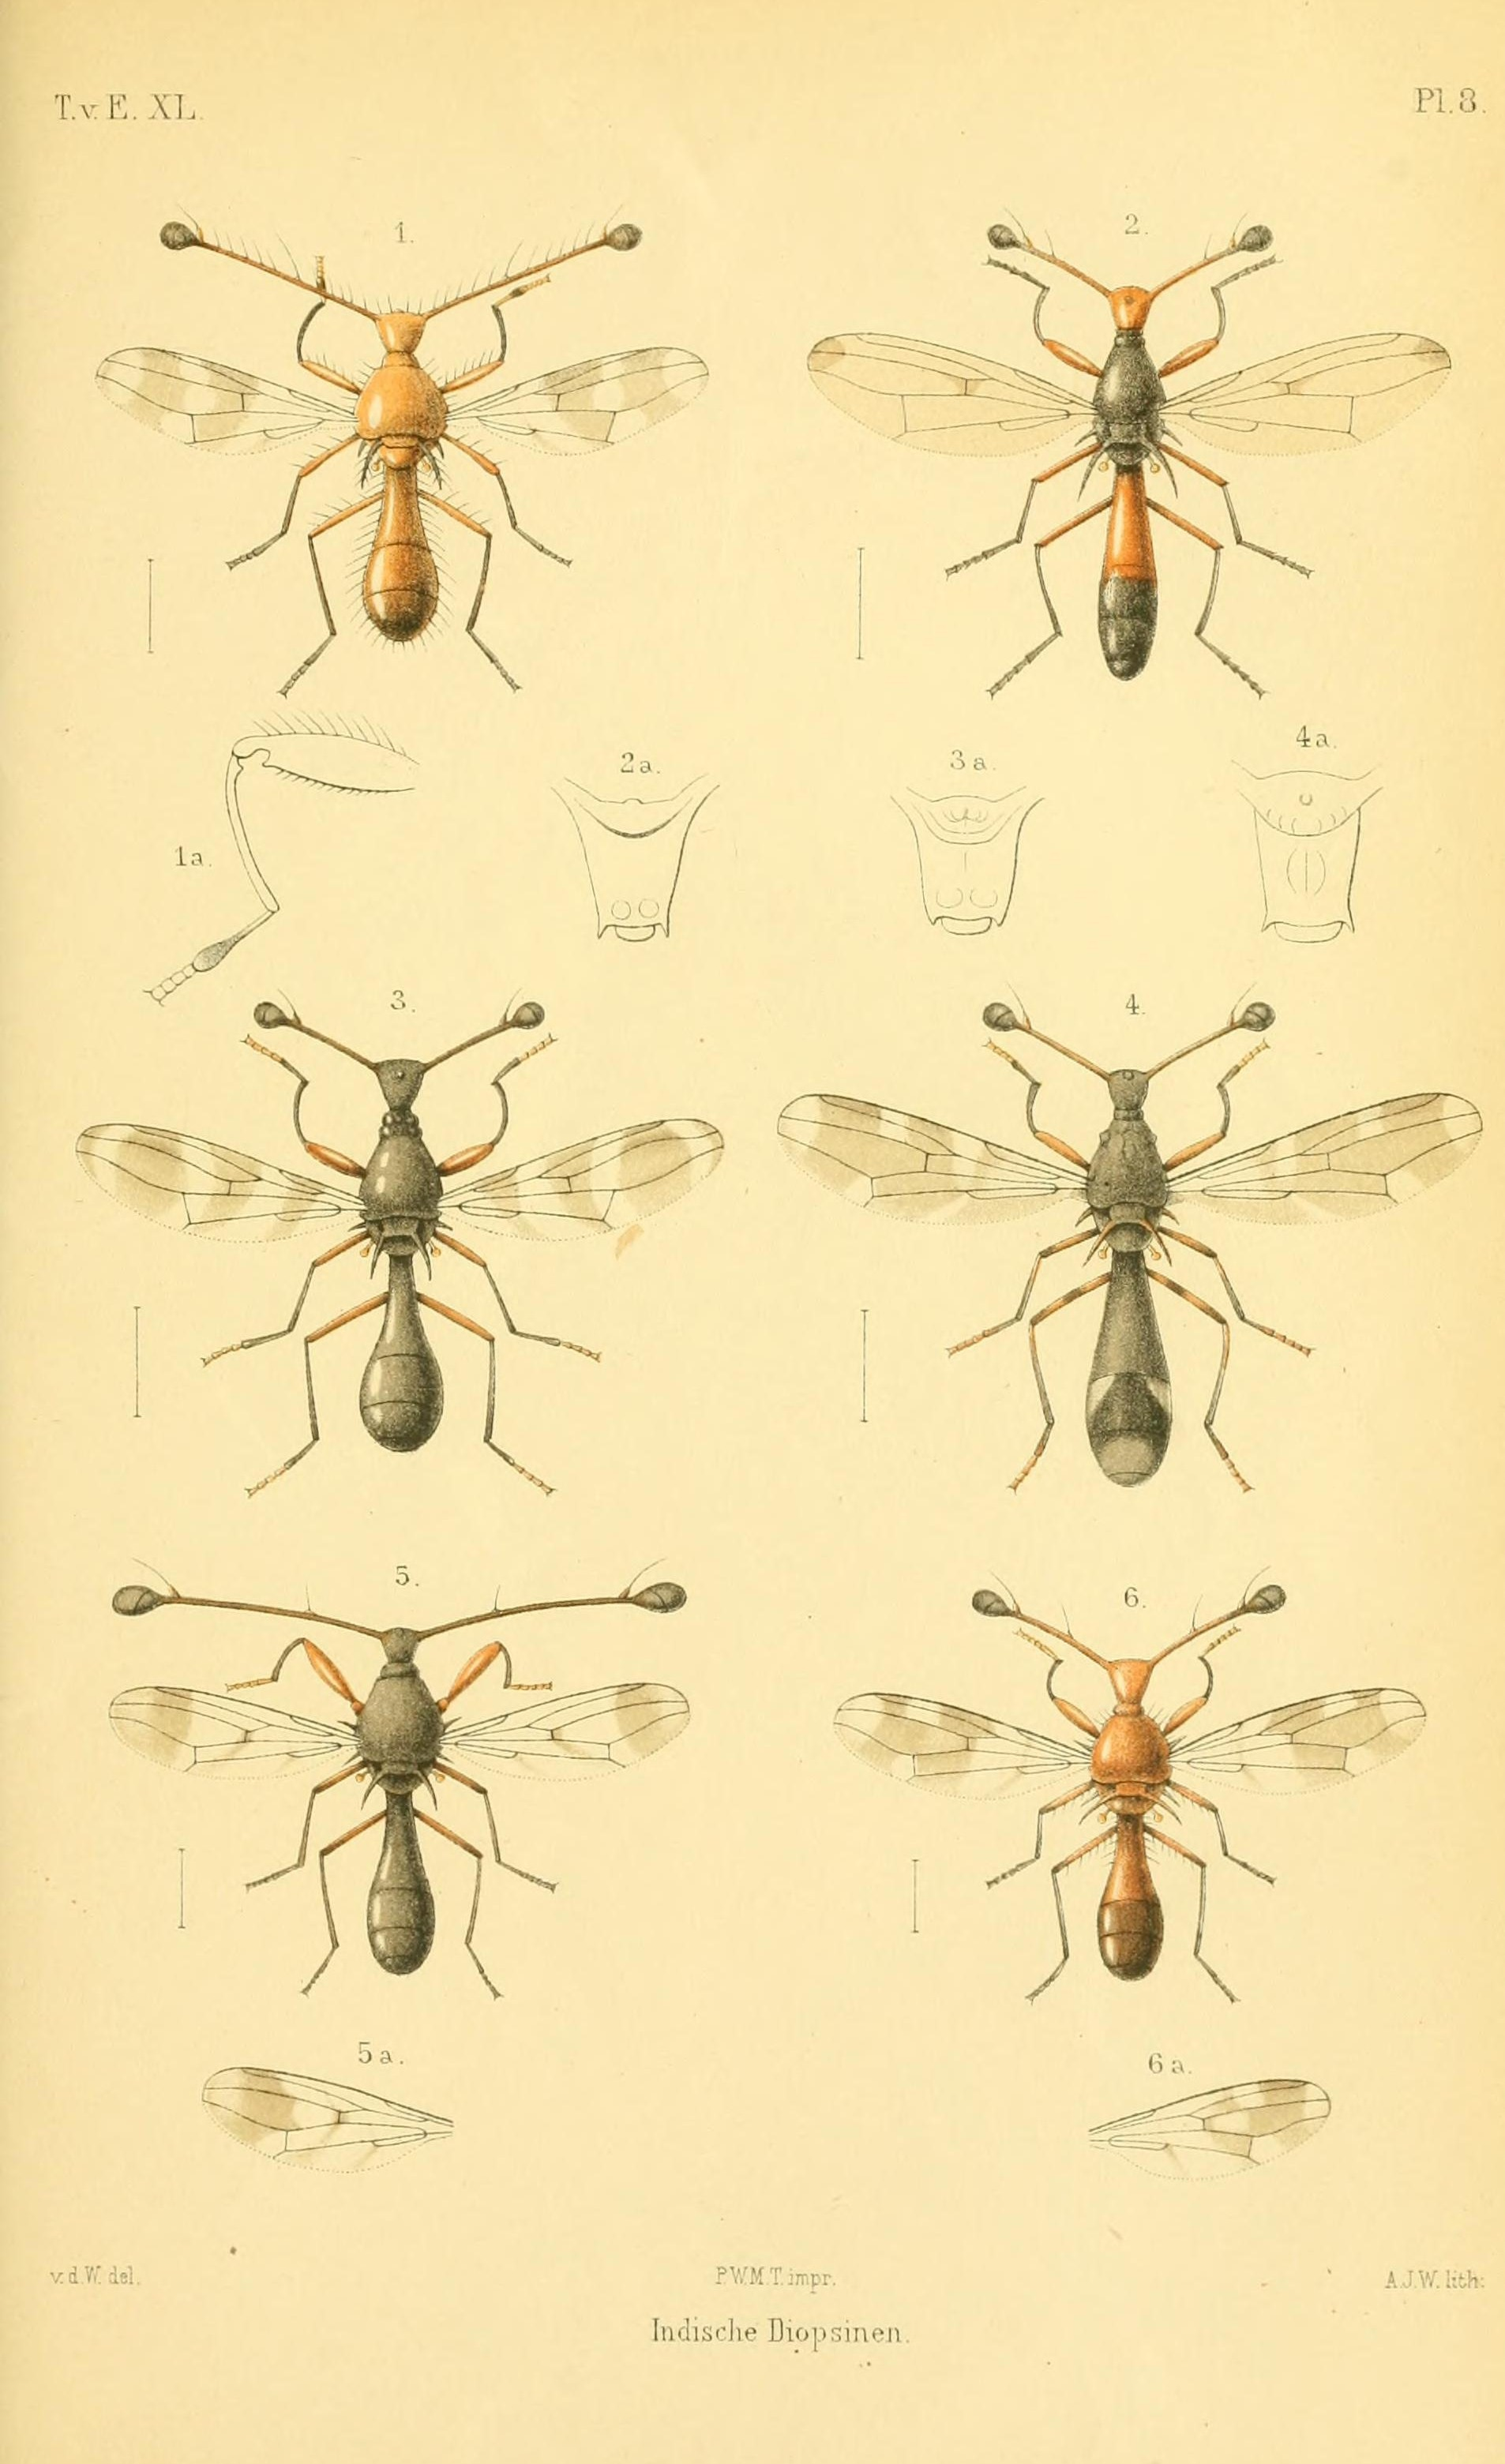
\includegraphics[width=0.9 \textwidth]{illustration_images/Quant_gen/Stalk_eyed_flies/WulpPlateVIIIjpg.jpg}
\end{center}
\caption{Stalk-eyed Flies ({\it Diopsidae}).  \BHLNC{Diptera. van der Wulp. 1898.}{https://www.biodiversitylibrary.org/item/39414\#page/631/mode/1up}{Smithsonian Libraries}} \label{fig:Stalk_eyed_flies}  
\end{marginfigure}
\begin{question}

At the end of ten generations in \citeauthor{wilkinson:93}'s experiment (Figure
\ref{fig:Stalk_eyed_response}), the males from the up- and down-selected
lines had mean eye-stalk to body ratios of $1.29$ and $1.14$
respectively, while the females from the up- and down-selected lines
had means of $0.9$ and $0.82$. \\
{\bf A)} \citeauthor{wilkinson:93} estimated that by selecting the top/bottom 10 males, he had on average shifted the mean body ratio by 0.024 within
each generation. What is the male heritability of eye-stalk to body-length ratio?

{\bf B)} Assume that the additive genetic variance of male and female phenotypes are
equal and that there is no direct
selection on female body-proportion in this experiment, i.e. that all of
the response in females is due to correlated selection. Can you
estimate the male-female genetic correlation of the eye-stalk ratio? 
\end{question}

\begin{figure*}
\begin{center} 
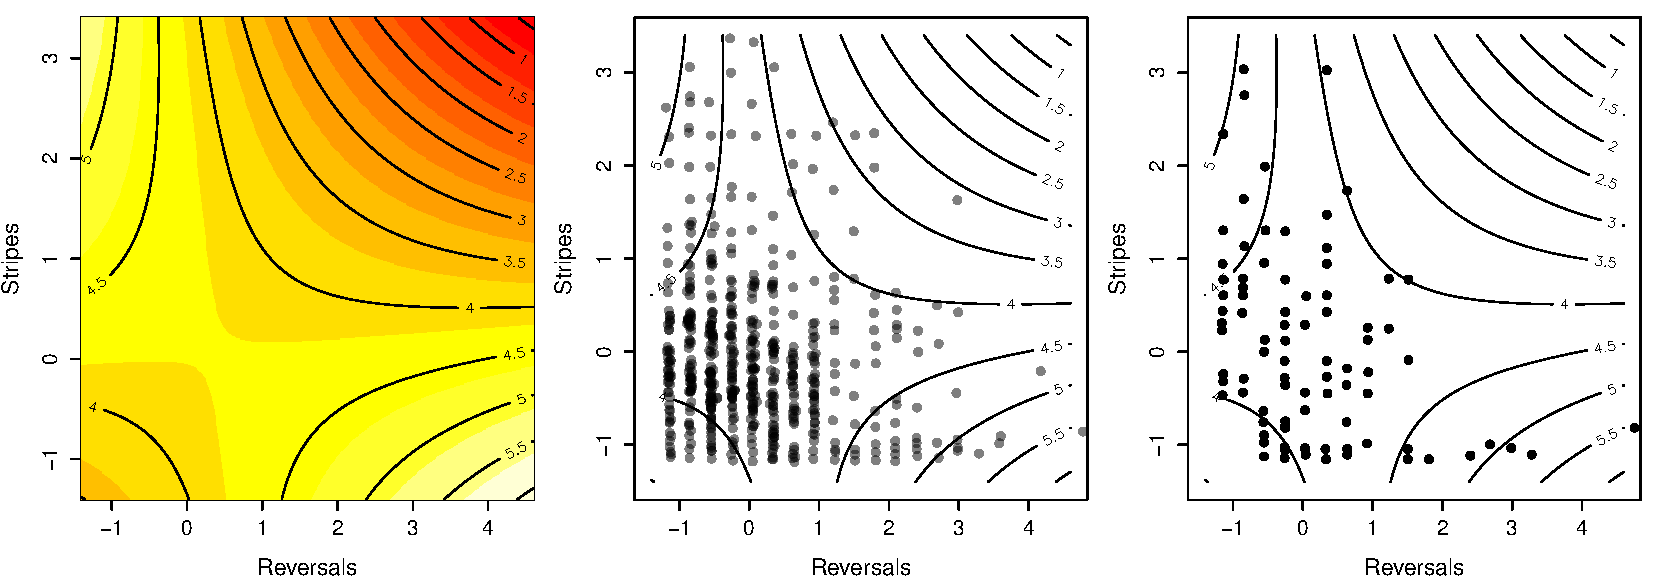
\includegraphics[width= \textwidth]{Journal_figs/Quant_gen/Garter_snakes_Brodie/Garter_snakes_Brodie.pdf}
\end{center}
\caption{ {\bf Left)} The garter snake fitness surface estimated by \citet{brodie1992correlational}
 lighter colours indicate higher
 relative fitness. {\bf Middle)} The phenotypes of all of the snakes released
   by Brodie, each dot is an individual. {\bf Right)} The phenotypes
   of surviving snakes. Note how snakes in the top left and bottom
   right corner are over represented in the survivors. Data from  \citet{brodie1992correlational}
  \gitcode{https://github.com/cooplab/popgen-notes/blob/master/Journal_figs/Quant_gen/Garter_snakes_Brodie/Garter_snakes_Brodie.R}. } \label{fig:Garter_snakes_Brodie}
\end{figure*} 

%s, where the snakes with thehighest probability of survival perform uninterrupted flight if striped but flee evasivelyif spotted or unstriped.  

% Eutaenia ordinoides
% northwestern garter snake (Thamnophis ordinoides)
%https://commons.wikimedia.org/wiki/File:The_natural_history_of_Washington_territory,_with_much_relating_to_Minnesota,_Nebraska,_Kansas,_Oregon,_and_California,_between_the_thirty-sixth_and_forty-ninth_parallels_of_latitude,_being_those_(14574590600).jpg

\paragraph{Estimating multivariate selection gradients}
We can estimate multivariate directional ($\beta$) and quadratic selection
gradients ($\gamma$) just as we did for a single traits ($x_1$ and $x_2$), using linear
and quadratic models (in eqn \eqref{fitness_regression} and \eqref{fitness_regression_stab}). For example, for two traits we can write
\begin{equation}
w_i \sim \beta_1 x_{1,i} + \nicefrac{1}{2} \gamma_1 x_{1,i}^2 + \beta_2 x_{2,i} + \nicefrac{1}{2} 
\gamma_2 x_{2,i}^2  + \gamma_{1,2} x_{1,i} x_{2,i}  + \wbar \label{fitness_regression_MV}
 \end{equation}
where $\beta_1$ and $\gamma_1$ are the directional and quadratic
selection gradients for trait one, and similarly for trait two \citep{lande1983measurement}. The
covariance selection gradient between traits is given by
$\gamma_{1,2}$ . This technique for measuring multivariate selection is
sometimes called `Lande-Arnold regression'.

\citet{brodie1992correlational}'s work provides a nice example of
selection on multiple predation-avoidance traits in northwestern garter snakes
({\it Thamnophis ordinoides}). \citeauthor{brodie1992correlational} released hundreds on snakes born in
the lab into the wild, and then performed mark-recapture observations
to monitor their fate.
\begin{marginfigure}
\begin{center} 
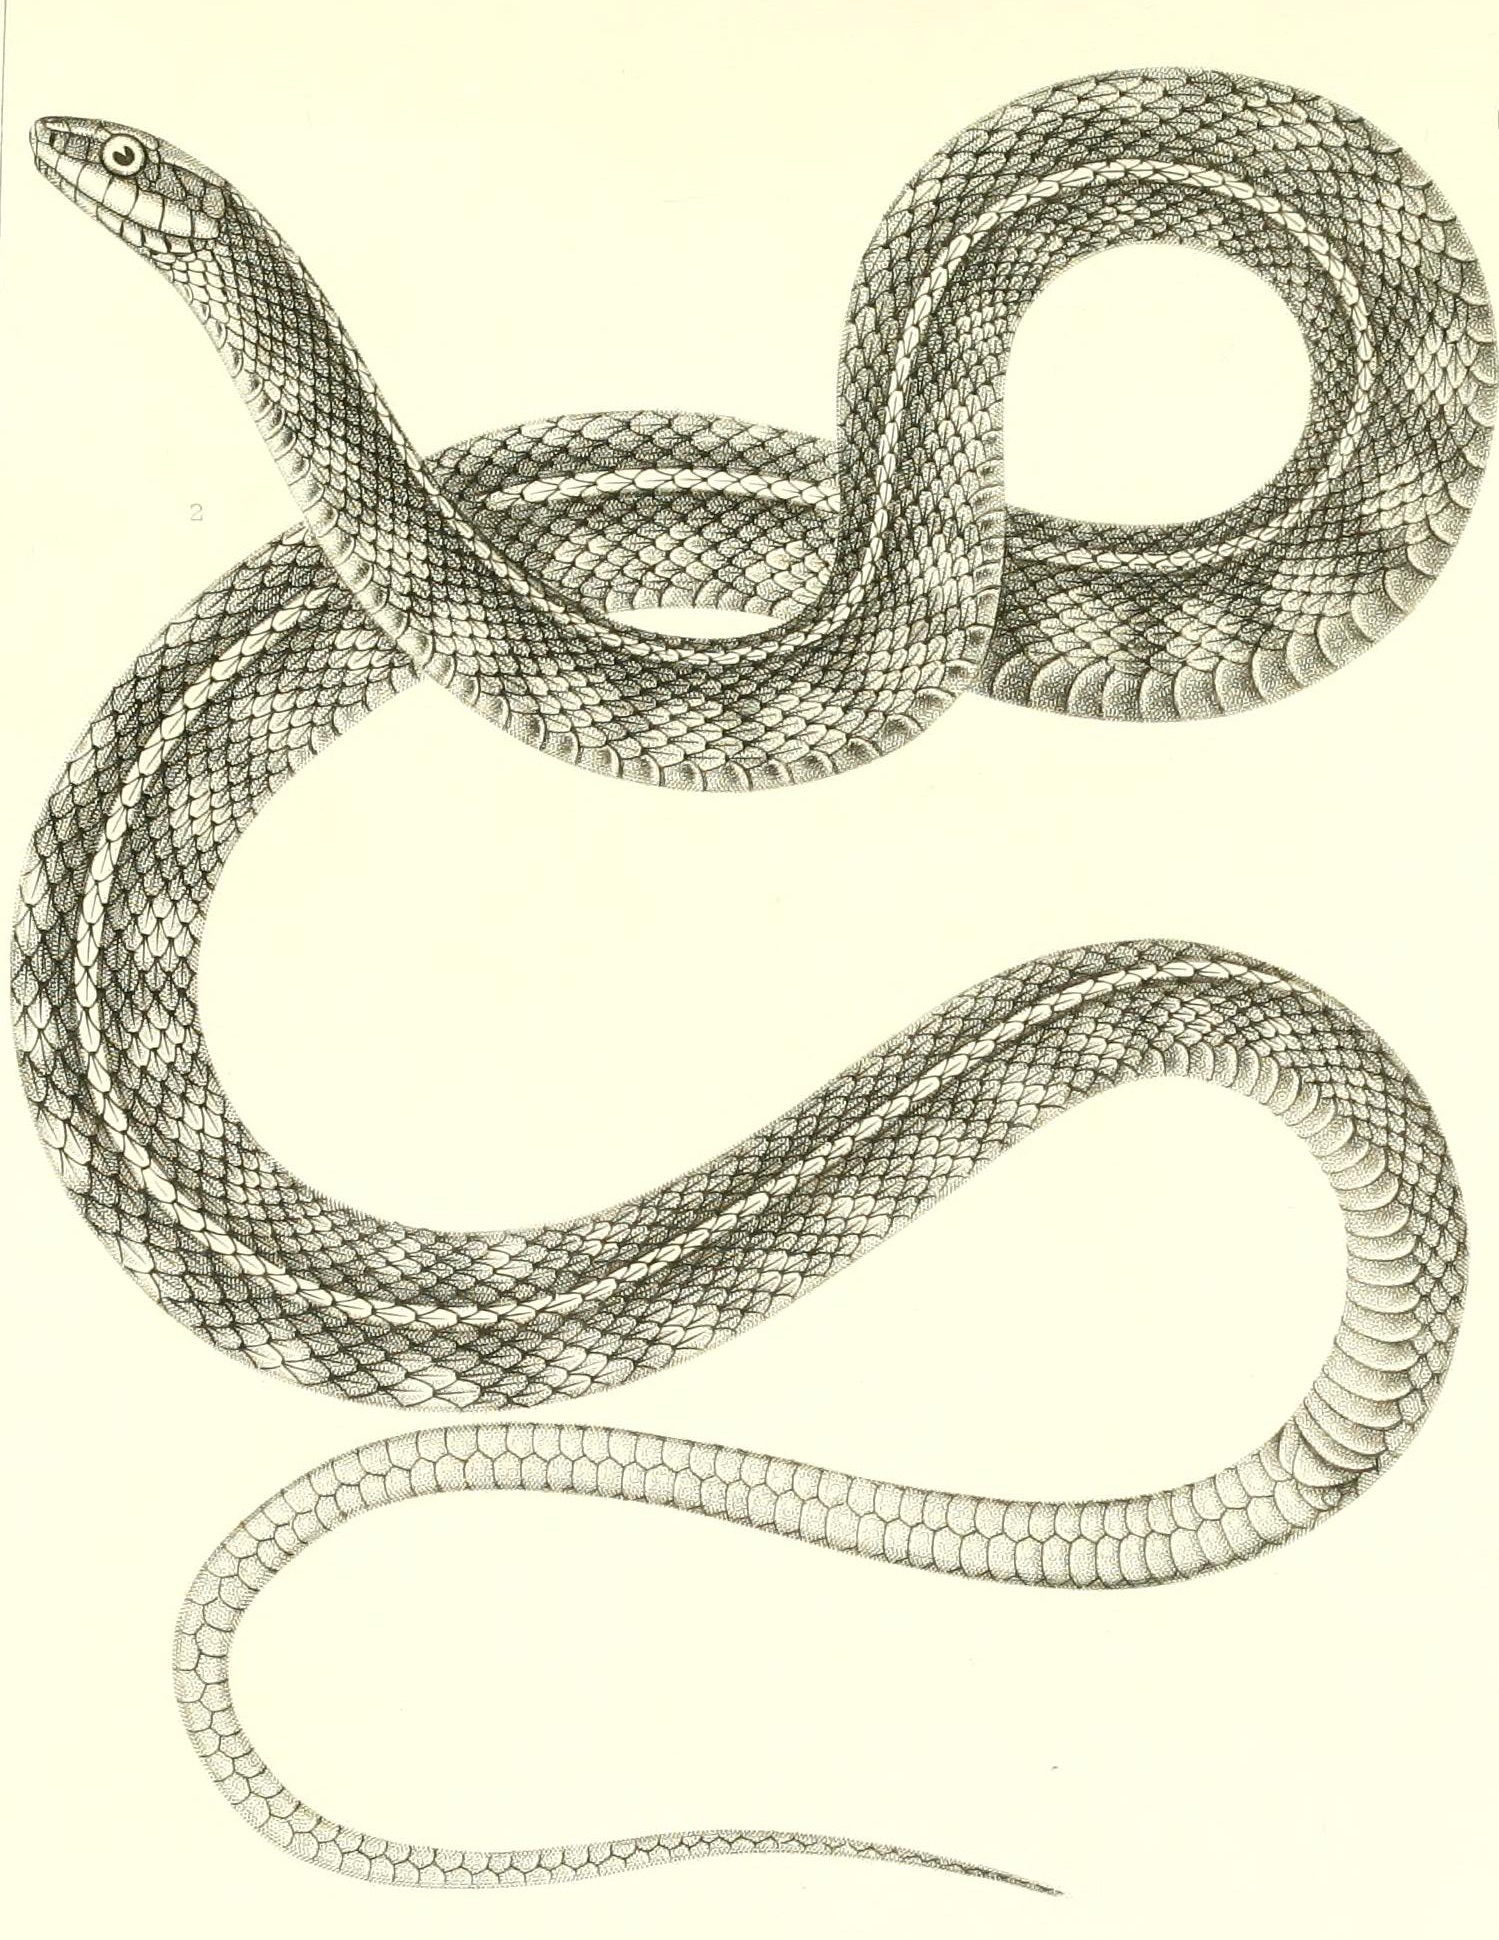
\includegraphics[width= 0.75\textwidth]{illustration_images/Quant_gen/Garter_snake/Eutaenia_cooperi.jpg}
\end{center}
\caption{Northwestern garter snake ({\it Eutaenia cooperi}, now {\it
    Thamnophis ordinoides})
\BHLNC{The natural history of Washington territory, with much relating to
  Minnesota, Nebraska, Kansas, Oregon, and California (1859). Cooper
  J.G. and Suckley,
  G. }{https://commons.wikimedia.org/wiki/File:The_natural_history_of_Washington_territory,_with_much_relating_to_Minnesota,_Nebraska,_Kansas,_Oregon,_and_California,_between_the_thirty-sixth_and_forty-ninth_parallels_of_latitude,_being_those_(14574590600).jpg}{Smithsonian
  Libraries} } \label{fig:Garter_snake}
%, between the thirty-sixth and forty-ninth parallels of latitude, being those parts of the final reports on the survey of the Northern Pacific railroad route, containing the climate and physical geography, with full catalogues and descriptions of the plants and animals collected from 185 to 1857
\end{marginfigure}  Before releasing them he measured how stripy
they were, and their behavioural tendency to reversals of direction
during simulated flight from a predator. His quadratic fitness surface is shown in Figure
\ref{fig:Garter_snakes_Brodie}, based on fitting the
regression given by eqn \eqref{fitness_regression_MV} to juvenile
survival. He found that neither single trait directional of quadratic
gradients were significant, ie there was no apparent selection on one 
trait ignoring the other. However, there was a significant, negative
covariance ($\gamma_{1,2}<0$). The individuals with the highest chance of survival are
{\it either} highly striped and perform few reversals (top left
corner), {\it or} have little striping but reverse course frequently
(bottom right corner). 

\gc{Add section of multivariate fitness landscapes}

\section{Some applications of the multivariate trait breeder's equation}

The multivariate breeders equation has a lot of different uses in
understanding the response of multiple traits to selection. It also
offers strong insights into the mechanistic underpinnings of kin selection and sexual selection. We'll discuss these next.

\subsection{Hamiliton's Rule and the evolution of altruistic and selfish behaviours}
\marginnote{\citet{smith1964kin} coined the name kin selection to describe Hamilton's approach to this problem. It's also sometimes called the inclusive fitness approach, as we need to include not just one individual's fitness but the weighted sum of all the fitness of all their relatives. }
Individuals frequently behave in ways that sacrifice their own fitness for the
benefit of others. That selection favours such apparent acts of altruism is puzzling at first sight. \citet{hamilton1964genetical,hamilton1964genetical2} supplied the first general evolutionary explanation of such altruism. 
His intuition was that while an individual is losing out of some reproductive output, the alleles underlying an altruistic behaviour can still spread in the population if this cost is outweighed by benefits gained 
through the transmission of these alleles through a related individual. Note that this means that the
allele is not acting in an self-sacrificing manner, even though individuals may as a result. 
 \begin{marginfigure}
\begin{center}
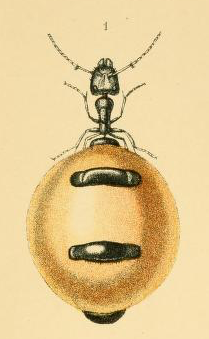
\includegraphics[width= 0.7 \textwidth]{illustration_images/Quant_gen/honey_ant/honey_ant.png}
\end{center}
\caption{Australian Honey-pot Ant ({\it Camponotus inflatus}). Honey ants are gorged with
  honeydew collected by their nest mates, till they swell to the size
  of grapes, and used as a food storage
  device.  \BHLNC{Ants,
  bees, and wasps; a record of observations on the habits of the
  social Hymenoptera (1897) Lubbock, J.}{https://www.biodiversitylibrary.org/page/9657360\#page/485/mode/1up}{Smithsonian Libraries}  } \label{fig:honey_ant}
\end{marginfigure} 

Altruism reflects social interactions. So as a simple model let's imagine that individuals interact in pairs, with our focal
individual $i$ being paired with an individual $j$. This could be pairs of siblings interacting.   
Imagine that individuals have two possible phenotypes $X=1$ or $0$,
corresponding to providing or withholding some small act of `altruism'
(we could just as easily flip these labels and call them an unselfish
act and a selfish act respectively). 
Our pairs of individuals interacting could, for example, be siblings sharing a
nest. The altruistic trait could be as simple as growing at a slightly slower rate so as to reducing sibling-competition for food from
parents, or more complicated acts of altruism such as children foregoing their own reproduction so as to help their parents raise their siblings.

Providing the altruistic act has a cost $C$ to the fitness of our individual and failing to provide this act has no cost. Receiving this altruistic act confers a fitness benefit $B$ over individuals who did not receive this act. \citeauthor{hamilton1964genetical}'s rule states that such a trait will spread through the population if 
\begin{equation}
 2F B > C 
\end{equation}
where $F$ is the average kinship coefficient between the interacting
individuals ($i$ and $j$). In the usual formulation of Hamilton's Rule our $2F$ is replaced by the `Coefficient of relationship', which is the
  proportion of alleles shared between the individuals. Here we use
  two times the kinship coefficient to keep things inline with our 
  notation for these chapters. Note that if our individuals are themselves inbred we need
to do a little more careful to reconcile these two measures.
So the altruistic behaviour will spread even if it is costly to the individual if its cost is paid off by the benefit to sufficiently related individuals. 

As one example of kin-selection consider \citet{krakauer2005kin}'s work on
co-operative courtship in wild turkeys ({\it Meleagris
  gallopavo}). Male turkeys often form display
partnerships, with a subordinate male helping a dominant male with
displaying to females and defending the females from other groups of males. \begin{marginfigure}
\begin{center}
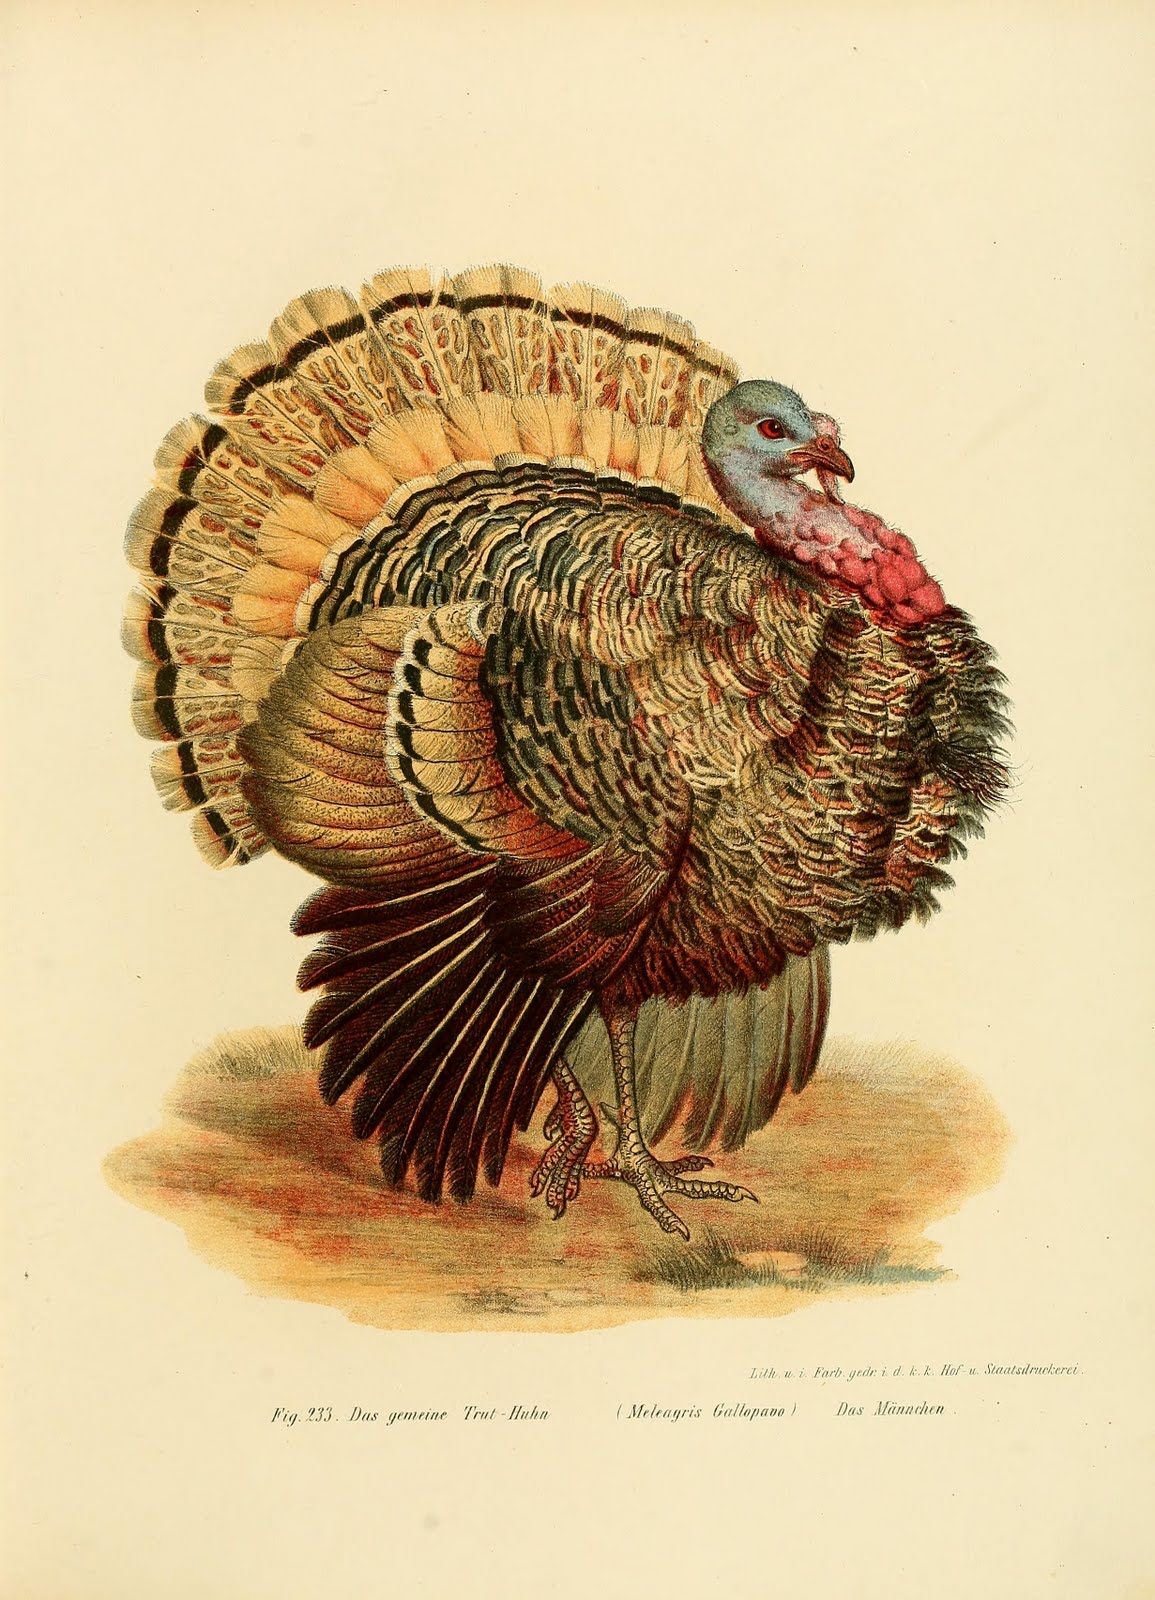
\includegraphics[width= \textwidth]{illustration_images/Quant_gen/Turkey/turkey.jpg}
\end{center}
\caption{Turkey  ({\it Meleagris
  gallopavo}). \BHLNC{Bilder-atlas zur Wissenschaftlich-populären
Naturgeschichte der Vögel in ihren sämmtlichen Hauptformen (1864). Wien,K.K. Hof}{https://www.biodiversitylibrary.org/page/33050564\#page/199/mode/1up}{Smithsonian Libraries} } \label{fig:turkey}
\end{marginfigure}  These pairs are often full brothers ($F=0.25$),
with the subordinate male often being the younger of the two. The
subordinate male often loses out on mating opportunities over their
entire lifetime by acting as a wingman to their older 
brothers. \citet{krakauer2005kin} estimated that dominant males gained
an extra $6.1$ offspring when they display with a partner than males
who display alone. While the subordinate males lose out on fathering $0.9$
offspring compared to solitary males. Thus the costs of helping by
subordinate males is more than compensated by the fitness gains of
their brothers ( $ (2 \times 0.25)  \times 6.1 > 0.9$), and so the
evolution of this  altruistic  helping in co-operative courtship is potentially well explained by kin-selection \citep[see ][for more analysis]{akccay2016}.
\begin{question}
How would this answer be changed if the male Turkey partnerships were only
$\nicefrac{1}{2}$ sibs, or first cousins?
\end{question}


\begin{marginfigure}
\begin{center}
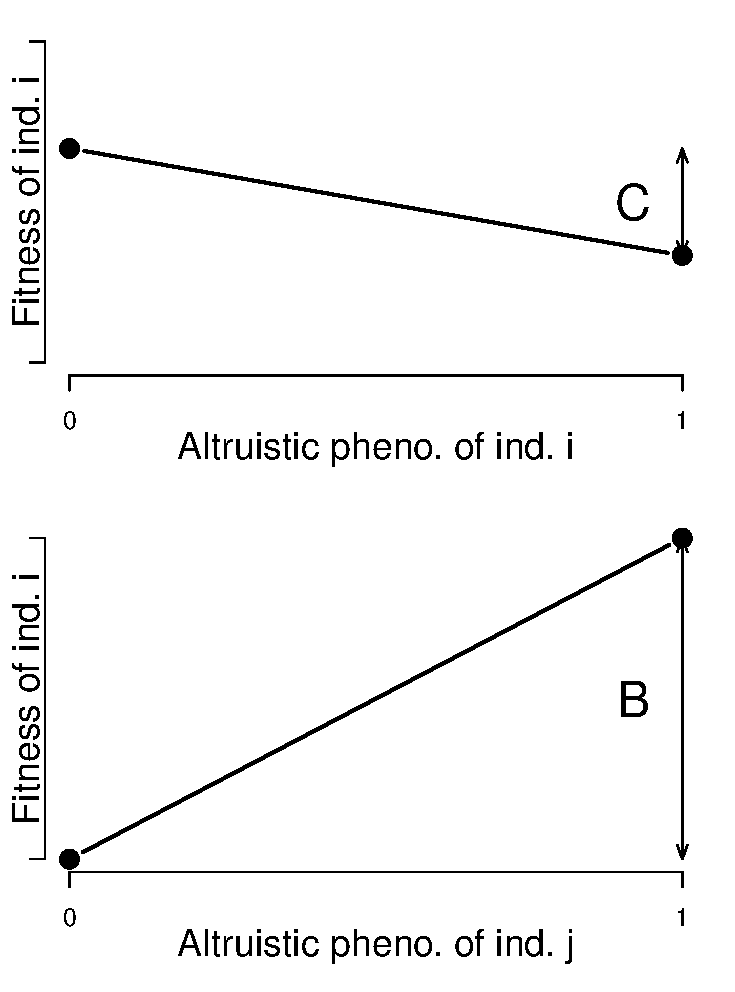
\includegraphics[width= \textwidth]{figures/Response_to_sel/Hamiltons_rule_B_C.pdf}
\end{center}
\caption{{\bf Top)} The fitness of individual $i$ as a function of
  their behavioural phenotype, where altruistic/non-altruistic
  behavioural phenotypes are encoded as $1$ and $0$ respectively. The
  direct fitness cost of behaving altruistically is $C$. {\bf Bottom)}
  The fitness of our focal individual $i$ as a function of the
  behavioural phenotype of their interacting partner ($j$). Our focal
  individual gets an increase $B$ in fitness if their partner behaves
  altruistically. \gitcode{https://github.com/cooplab/popgen-notes/blob/master/Rcode/Quant_gen/Hamilton_rule_B_C.R}} \label{fig:Hamilton_B_C}
\end{marginfigure}


Where does this result come from? Well, we can use our quantitative genetics framework to gain some 
intuition by deriving a simple version of Hamilton's Rule by thinking
about the phenotypes of an individual's kin as genetically correlated
phenotypes. To sketch a proof of this result, let's assume that our focal $i$ individual's fitness can be written as 
\begin{equation}
W(i,j)= W_0 + W_i +W_j
\end{equation}
where $W_i$ is the contribution of the fitness of the individual $i$ due
to their own phenotype, and $W_j$ is the contribution to our
individual $i$'s fitness due to the interacting individual $j$'s behaviour (i.e. $j$'s phenotype).
With the benefit $B$ and cost $C$, our $W(i,j)$ are depicted in Figure \ref{fig:Hamilton_B_C}. 

Following our multivariate breeder's equation, we can write the expected change of our behavioural phenotype as 
\begin{equation}
R = \beta_i V_A + \beta_j V_{A,i,j},
\end{equation}
Our altruistic phenotype is increasing in the population if $R>0$, i.e. if 
\begin{equation}
  \beta_i V_A + \beta_j V_{A,i,j}  > 0 \end{equation}
\marginnote{ Here we've following a simplified version of
  \citet{queller1992quantitative}'s treatment, to re-derive Hamilton's rule in a quantitative genetics framework (Hamilton's original papers did this in a population genetics framework).} The slope $\beta_i$ of the regression of our focal individual's
behavioural phenotype on fitness is proportional to $-C$. The slope
$\beta_j$ of the regression of our interacting partner's phenotype on
our focal individual's fitness is proportional to $B$ (with the same
constant of proportionality). Therefore, our altruistic phenotype is increasing in the population if
\begin{eqnarray}
  \beta_i V_A + \beta_j V_{A,i,j} & > 0  \nonumber  \\
 B \frac{V_{A,i,j}}{V_A} & >  C
\end{eqnarray}
So what's the average genetic covariance between
individual $i$ and $j$'s altruistic phenotype? Well it's the same behavioural phenotype in both individuals, so the phenotypes are genetically correlated if our individuals are related to each other. The covariance of the same phenotype between two individuals is just $2 F_{i,j} V_A$ (see \eqref{additive_covar_general_rellys}). So our altruistic phenotype is increasing in the population if 
\begin{eqnarray}
   & B\frac{2 F_{i,j} V_A}{V_A} &> C \nonumber  \\
  2 F_{i,j} B & > C 
\end{eqnarray}

Seen from this perspective, \citeauthor{hamilton1964genetical}'s rule
is simply a statement that altruistic behaviours can spread via
kin-selection, if the average cost to an individual of displaying an
altruistic phenotype, i.e. carrying altruistic alleles, is paid back through the average benefit of interacting with altruistic relatives (kin).


%\erin{this phrasing is a little misleading because it's 'paid back' to the allele, but not to the individual. I'd suggest something like 'if the fitness cost of altruism to an allele is paid back on average through the benefits of interacting with altruistic relatives (kin).


% Special eg on kinship, good for other egs https://www.cell.com/current-biology/issue?pii=S0960-9822(18)X0012-8

\subsection{Sexual selection and the evolution of mate preference by indirect benefits. }


Organisms often put an enormous effort into finding and attracting mates, sometimes at
a considerable cost to their chances of survival. Why are individuals so choosy about who they mate with, particularly when their choice seems to be based on elaborate characters and arbitrary displays
that surely lower the viability of their mates?  

\begin{marginfigure}[-8cm]
\begin{center}
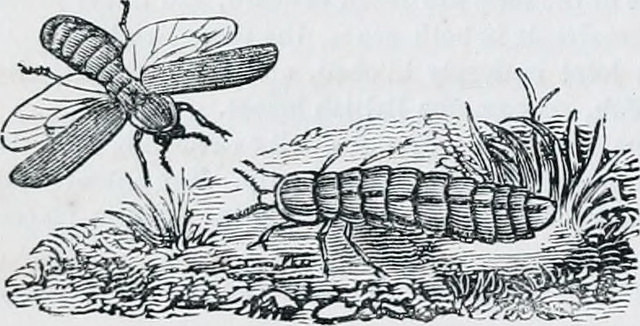
\includegraphics[width= \textwidth]{illustration_images/Quant_gen/glow_worm/18011950889_b2a1a1323e_z.jpg}
\end{center}
\caption{Male (left) and female (right) common glow worm  ({\it Lampyris
    noctiluca}). \BHLNC{The animal kingdom : arranged after its organization;
  forming a natural history of animals, and an introduction to
  comparative anatomy. (1863) Cuvier, G.}{https://www.flickr.com/photos/internetarchivebookimages/18011950889/in/photolist-Uqr16w-UqqZZu-4VxYcU-ZiyCTu-8DEFyz-6pxZpd-ZiyCXC-yFyBF-GEoD6s-u3DKnd-6pxZrd-4q7euj-5KsWen-yqphkW-xvGrfw-ytA3rP-ybfeBA-yqi7oo-tFL3h3-xvJnrz-BPm4Jd-wLVg9F-trDXtp-wVbxw2-y6MpEq-BWCQVA-vb793E-tHGekh-u4av2t-oewQcC-ow671H-t6ZJg7-u4Ap1m-xntXw9-ovPEMu-u3DFws-vbeMw2-tHMJiY-u1FJpo-tLqTCw-fFFAEG-y1Pfmz-u1FHaE}{University of Toronto - Gerstein Science Information Centre} } \label{fig:glow_worms}
\end{marginfigure}

\begin{marginfigure}[-2cm]
\begin{center}
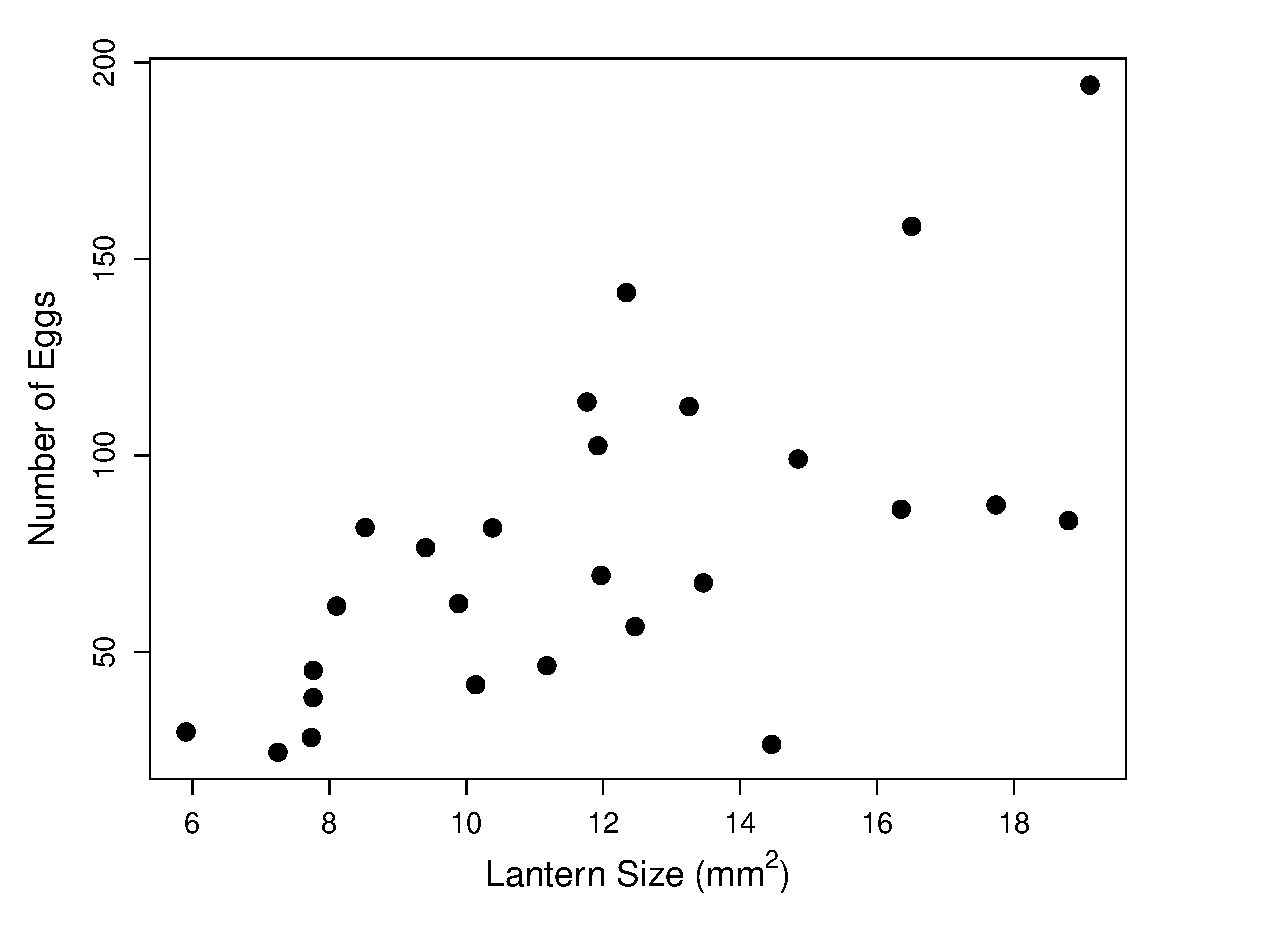
\includegraphics[width= \textwidth]{Journal_figs/Quant_gen/glow_worm_flashes/glow_worm_flashes.pdf}
\end{center}
\caption{Female Glow worms who have the largest, and therefore
  brightest, lanterns have the highest fecundity. Data from
  \citet{hopkins2015m}. \gitcode{https://github.com/cooplab/popgen-notes/blob/master/Journal_figs/Quant_gen/glow_worm_flashes/glow_worm_flashes.R} } \label{fig:glow_worms_lantern}
\end{marginfigure}


One major reason why individuals evolve to be choosy about who they mate with is that it can directly impact their fitness. By choosing a mate with
particular characteristics, individuals can gain more parental care for
their offspring, avoid parasites, or be choosing a mate with higher fertility. For example,  female glow-worms flash at night to attract males flying by. Females with larger, brighter lanterns have higher fecundity, so
males with a preference for brighter flashes will gain a direct benefit to their own fitness. (Note that males will benefit even if these differences in female fecundity are entirely driven by differences in environment, and so non-heritable.) Indeed male glow worms have evolved to be attracted to brighter
flashing lures.  

However, even in the absence of direct benefits of choice, selection can still indirectly favour the evolution of choosiness. These
indirect benefits occur because individuals can have higher fitness
offspring by choosing a mate whose phenotype indicates high viability
(the so-called good genes hypothesis), or by choosing a mate whose
phenotype is simply attractive, and likely to produce similarly
attractive offspring (the `runaway' or sexy sons hypothesis).

We'll denote a display trait, e.g. tail length, in males by $\mars$ and a preference
trait in females by $\venus$. Our display trait is under direct selection in males, such that its response to selection can be written as
\begin{equation}
R_{\mars} = \beta_{\mars} V_{A, \mars}
\end{equation}
Let's assume that the female preference trait, the degree to which
females are attracted to long tails, is not under direct
selection $\beta_{\venus}=0$. Then the response to selection of the
preference trait can be written as
\begin{eqnarray}
R_{\venus} &=\beta_{\venus}V_{A,\venus}  + \beta_{\mars} V_{A, \venus
  \mars}
& = \beta_{\mars} V_{A, \venus  \mars}
\end{eqnarray}
So the female preference will respond to selection if it is
genetically correlated with the male trait, i.e. if $V_{A, \venus
  \mars}$ is not zero. There's a number of different ways this genetic correlation could arise; the
simplest is that the loci underlying the male trait may have a
pleiotropic effect on female preference. However, female preference
may often have quite a distinct genetic basis from male display traits.
\begin{figure}
\begin{center}
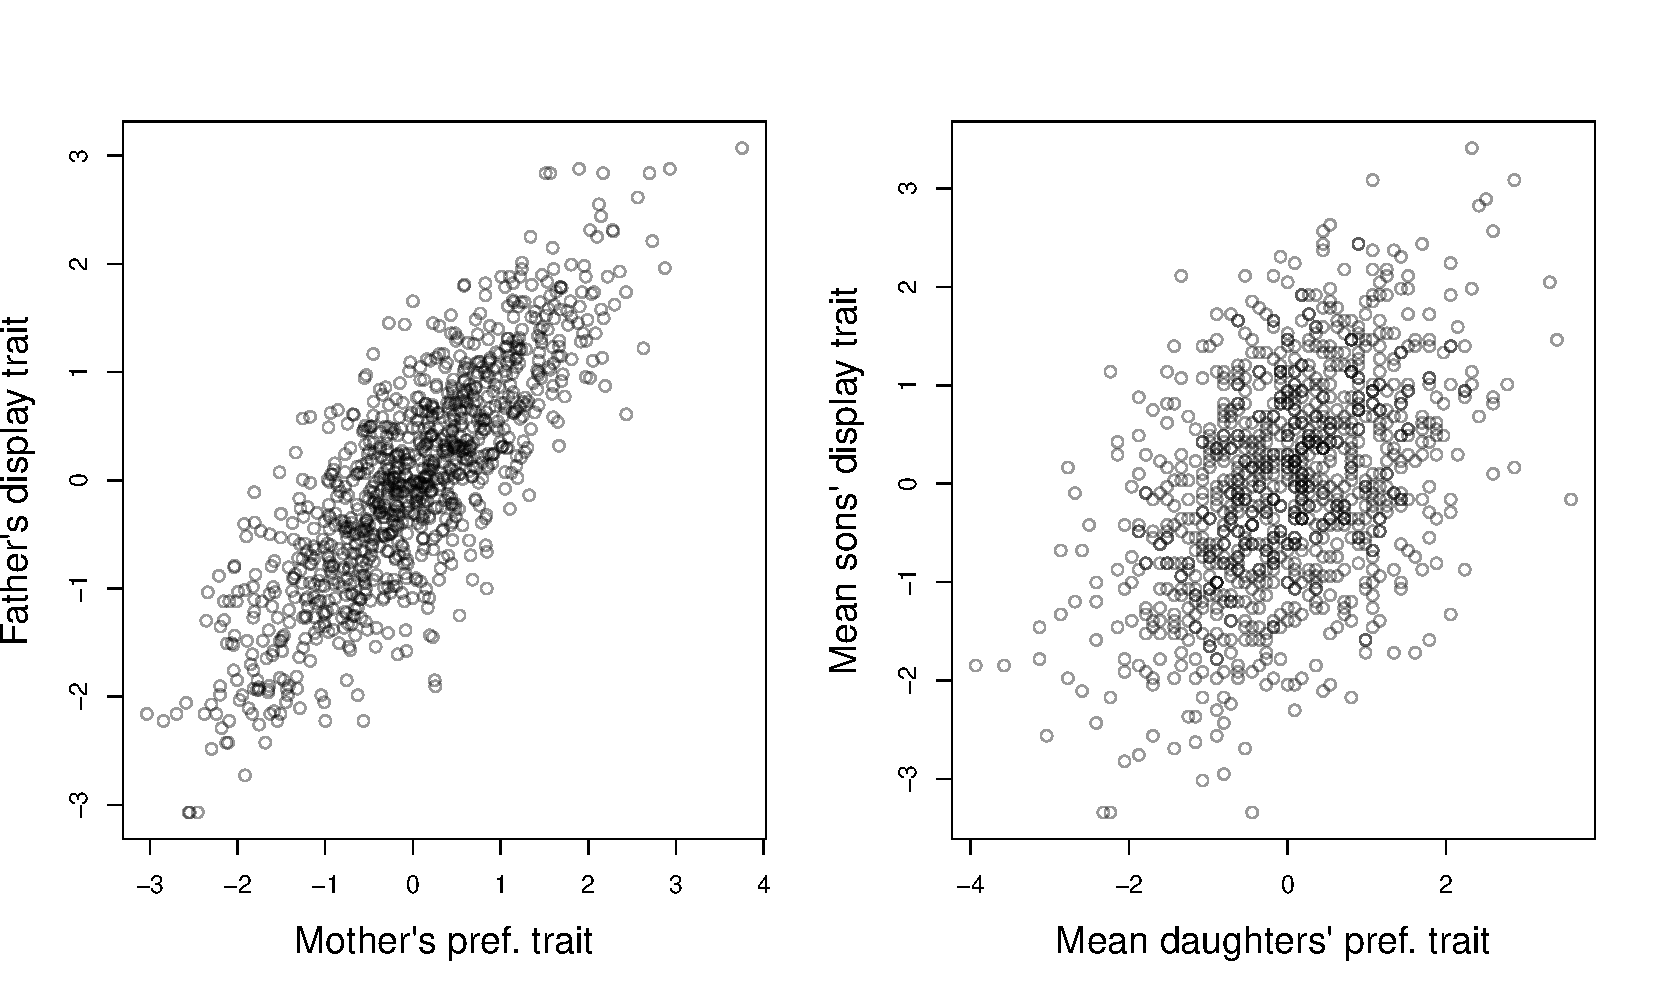
\includegraphics[width=\textwidth]{figures/Response_to_sel/Genetic_corr_assort_mating.pdf}
\end{center} \label{fig:assort_mating_2_trait}
\caption{{\bf Left)} Assortative mating between males and
  females. Males vary in a display trait (e.g. tail length), females
  vary in their preference for this trait. We see evidence of
  assortative mating as females with a preference for a particular
  value of the male trait tend to mate with those males. {\bf Right}) As both
  male trait and female preference are genetic this establishes a
  genetic correlation in the next generation. This is simulated data. \gitcode{https://github.com/cooplab/popgen-notes/blob/master/Rcode/Quant_gen/QT_cross_assortative_mating_2_kids.R}} \label{fig:assort_mating_2_trait}
\end{figure}

A more general way in which trait-preference genetic correlations may arise is through assortative mating. As females vary in their
tail-length preference, the ones with a preference for longer
tails will mate with long-tailed males and the opposite for females
with a preference for shorter-tails. Therefore, a
genetic correlation between mates display and preference traits will
become established (see Figure \ref{fig:assort_mating_2_trait}). 

The males with the longer tails will also carry the alleles
associated with the preference for longer tails, as their long-tailed
dads tended to mate with females with a genetic preference for long
tails. Similarly, the the males with shorter tails will carry alleles associated with the preference for
shorter tails. Thus if there is direct selection for males with longer tails, then
the female preference for longer tails will increase too, as it is
genetically correlated via assortative mating. 

\begin{figure}
\begin{center}
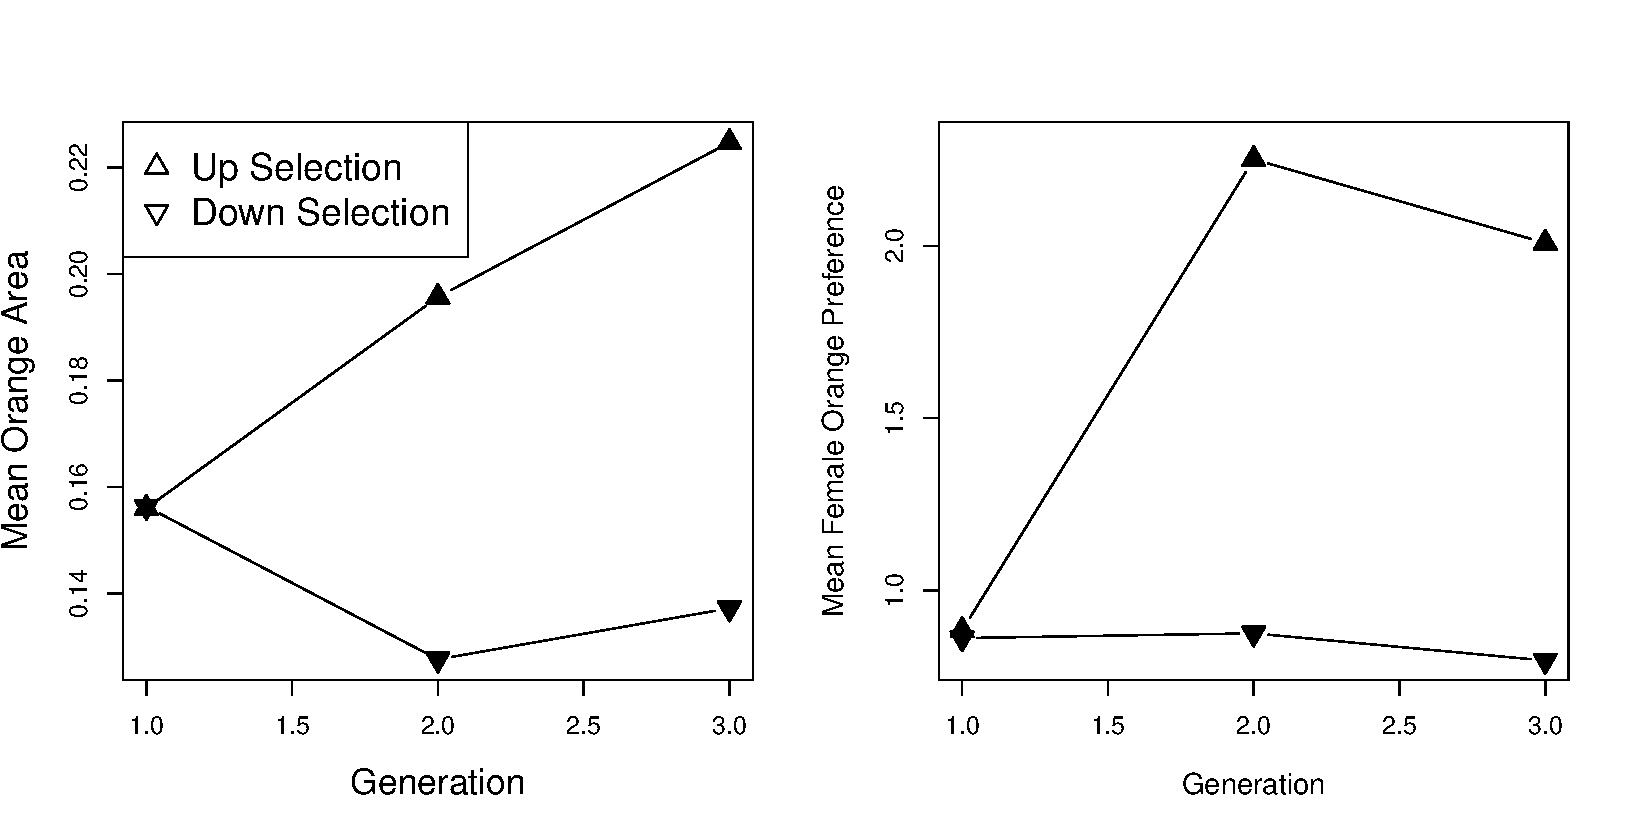
\includegraphics[width=\textwidth]{Journal_figs/Quant_gen/guppies_female_choice/guppies_female_choice.pdf}
\end{center} \label{fig:assort_mating_guppies}
\caption{Mean phenotypes for the two up- and two down-selected
  populations of Guppies. Left panel: A response to selection was seen
  due to the direct selection on male colouration. Right panel: An
  indirect, correlated response was also seen in female
  preference. Data from \citet{houde:94}. \gitcode{https://github.com/cooplab/popgen-notes/blob/master/Journal_figs/Quant_gen/guppies_female_choice/guppies_female_choice.R}}
\end{figure}

As an example of how direct selection on display traits can drive the
evolution of preference traits, let's consider some data from
guppies. Guppies ({\it Poecilia reticulata}) are a classic system for
studying the interplay of natural and sexual selection. In some populations of
guppies, females show a preference for males with more orange colouration.\begin{marginfigure}
\begin{center}
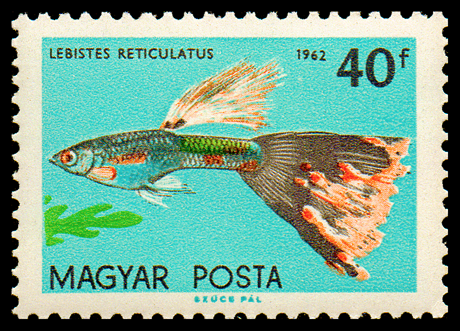
\includegraphics[width=\textwidth]{illustration_images/Quant_gen/Guppies/1439_fish_40.png}  %https://commons.wikimedia.org/wiki/File:1439_fish_40.png
\end{center} \label{fig:assort_mating_guppies}
\caption{Guppy ({\it Poecilia reticulata}). \newline \noindent \tiny{From a set of 1962 stamps
  of Hungary. Contributed to \href{https://commons.wikimedia.org/wiki/File:1439_fish_40.png}{wikimedia} by Darjac, not covered by copyright}}
\end{marginfigure} 
 \citeauthor{houde:94} established four replicate
population pairs of guppies and selected one of each pair for an increased or decreased orange coloration in males, selecting the top/bottom $20$ out of $50$
males. She randomly chose females from each population to form the next generation, and so did not
exert direct selection on females. She measured the response to 
selection on male colouration and on female preference for orange (left
and right panels of Figure \ref{fig:assort_mating_guppies}
respectively). In the lines that were selected for more orange males
females showed an increased preference for orange. While in those
lines that she selected males for less orange in their display females
showed a decreased preference for orange. This is consistent with indirect selection on female orange preference as a response to
selection on male colouration, due to a genetic correlation between
female preference and male trait. It is {\it a priori} unlikely
that pleiotropy is the source of the genetic correlation between these
traits, rather it is likely caused by females assortative mating with
males that match their colour preference. 




Returning to our bird tail example, what could drive the direct
selection on male tail length? The selection for longer tails in males could come about because
longer tails are genetic correlated with higher male viability, for
example perhaps only males who gather an excess of food have the
resources to invest in growing long tail, i.e. a long tail is an
honest signal. This would be a good genes explanation of female mate
choice evolution.  

\begin{marginfigure}
\begin{center}
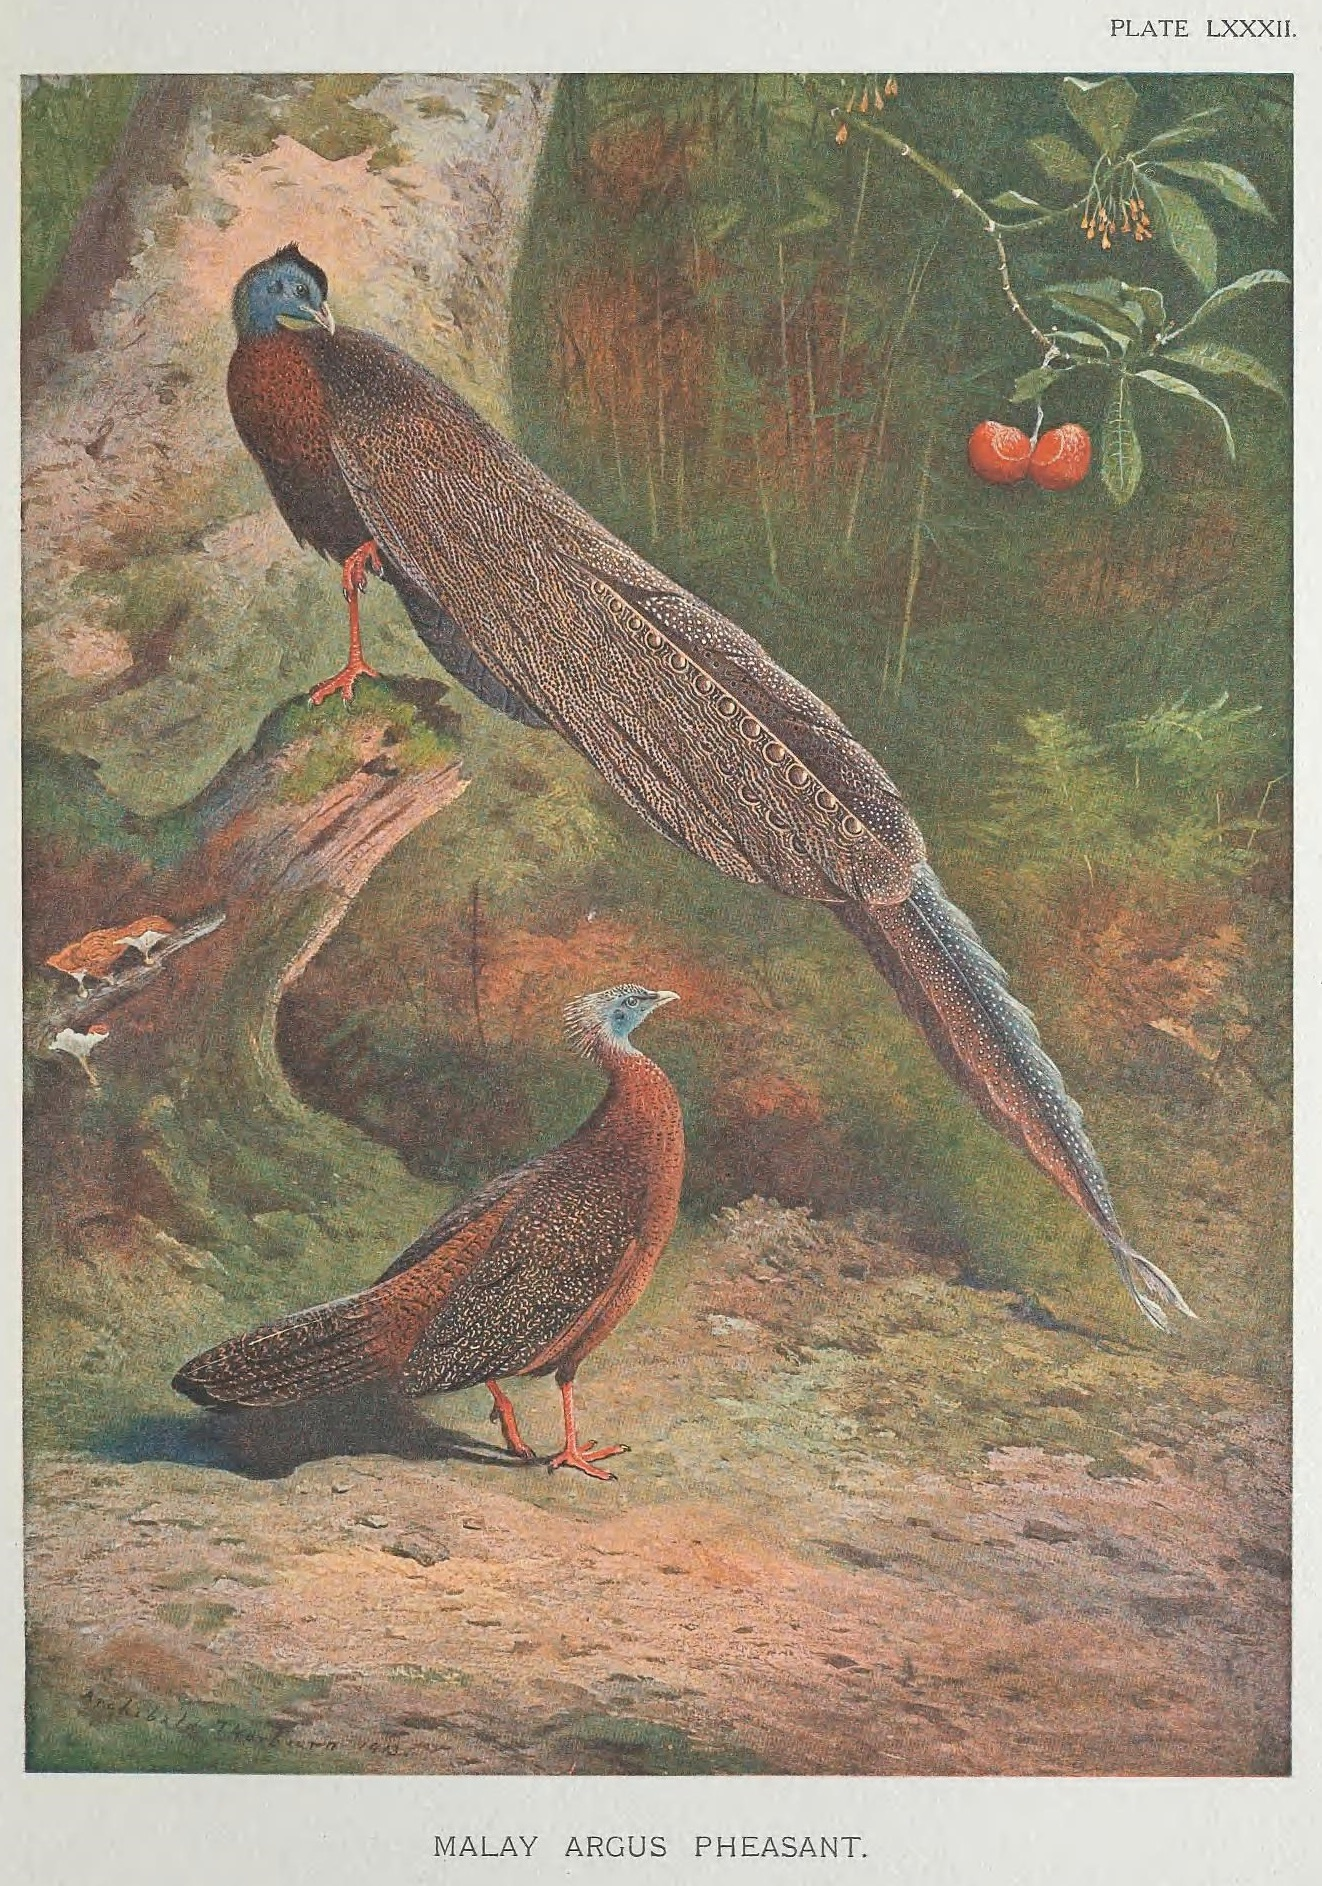
\includegraphics[width= \textwidth]{illustration_images/Quant_gen/Argus_pheasant/Argus_pheasant_small.jpg}
\end{center}
\caption{Argus Pheasant.  \BHLCC{A monograph of the pheasants. (1918). Beebe, W}{https://www.flickr.com/photos/biodivlibrary/10053909294/}{Smithsonian Institution Libraries}{2.0}} \label{fig:argus}
\end{marginfigure}
\marginnote{
\begin{quote}
``The case of the male Argus Pheasant is eminently interesting,
because it affords good evidence that the most refined beauty may
serve as a sexual charm, and for no other purpose.'' -- \citet{darwin1888descent}
\end{quote} }

There's another subtler way that selection could favour our male
trait. Imagine that the variation in female preference trait is
because some females have no strong preference for the male-tail
length, but some females have a strong preference for males with
longer tails. Males with longer tails would then have higher fecundity than
the short-tailed males as there's a subset of females who are strongly
attracted to long tails, and these males also get to mate with the
other females. Thus selection favours long-tailed males, and so indirectly favours
female preference for longer tails; females with a preference
for longer-tails have sons who in turn who are more attractive. This
model is sometimes called the sexy-son model. It is also called
the Fisherian runaway model \citep{fisher1915evolution}, as female
preference and male trait can coevolve in an escalating fashion
driving more and more extreme preferences for arbitrary traits. Thus
many extravagant display traits in males and females may exist purely
because individuals find them beautiful and are attracted to them. 



%\erin{I don't take away from this description that you can get runaway sexual selection without external directional selection for longer tails ... can you make that more clear? I think the problem is making the female trait a preference for short vs. long tails when maybe it should be presented as a preference for long tails vs. no preference so the males with longer tails get a boost from positive sexual selection. Also, why do you plot mean daughter's trait against mean son's trait and not, say, mean father's trait against mean daughter's trait or increase in population prevalence or correlation between male-female traits over time?}



% potential guppy image https://www.google.com/imgres?imgurl=https%3A%2F%2Fc1.staticflickr.com%2F1%2F457%2F20360503816_a88cdcd96d_b.jpg&imgrefurl=https%3A%2F%2Fwww.flickr.com%2Fphotos%2Finternetarchivebookimages%2F20360503816&docid=jtYRcc7UmAvIeM&tbnid=DBAauK0xAgK4mM%3A&vet=10ahUKEwirkrKWy8rcAhWTAHwKHfVdCmUQMwg2KAEwAQ..i&w=1024&h=840&itg=1&client=firefox-b-1-ab&bih=681&biw=1280&q=Lebistes%20reticulatus&ved=0ahUKEwirkrKWy8rcAhWTAHwKHfVdCmUQMwg2KAEwAQ&iact=mrc&uact=8
